\documentclass[a4paper,12pt]{report}

% ============================================================
% PACKAGES
% ============================================================
\usepackage{a4wide,amssymb,epsfig,latexsym,multicol,array,hhline,fancyhdr}
\usepackage[utf8]{inputenc}
\usepackage[T5]{fontenc}
\usepackage[vietnamese,english]{babel}
\usepackage{listings}
\usepackage{amsmath}
\usepackage{amsfonts}
\usepackage{lastpage}
\usepackage[lined,boxed,commentsnumbered]{algorithm2e}
\usepackage{enumerate}
\usepackage{enumitem}
\usepackage[table]{xcolor}
\usepackage{graphicx}
\usepackage{array}
\usepackage{makecell}
\usepackage{tabularx, caption}
\usepackage{longtable}
\usepackage{multirow}
\usepackage{multicol}
\usepackage{rotating}
\usepackage{float}
\usepackage[left=3cm, right=2cm, top=2.5cm, bottom=2.5cm]{geometry}
\usepackage{setspace}
\usepackage{tikz}
\usepackage{booktabs}
\usepackage{minted}
\usetikzlibrary{arrows,decorations.pathmorphing,backgrounds,shapes,positioning}
\usepackage{hyperref}
\hypersetup{urlcolor=blue, linkcolor=black, citecolor=black, colorlinks=true}
\usepackage{titlesec}
\usepackage{pdfpages}
\usepackage{indentfirst}

% ============================================================
% COLORS
% ============================================================
\definecolor{codegreen}{rgb}{0,0.6,0}
\definecolor{codegray}{rgb}{0.5,0.5,0.5}
\definecolor{codepurple}{rgb}{0.58,0,0.82}
\definecolor{backcolour}{rgb}{0.95,0.95,0.92}
\definecolor{darkblue}{RGB}{0,51,102}
\definecolor{hcmutblue}{RGB}{0,82,165}

% ============================================================
% CODE LISTING STYLE
% ============================================================
\lstdefinestyle{mystyle}{
    backgroundcolor=\color{backcolour},
    commentstyle=\color{codegreen},
    keywordstyle=\color{hcmutblue}\bfseries,
    numberstyle=\tiny\color{codegray},
    stringstyle=\color{codepurple},
    basicstyle=\ttfamily\footnotesize,
    breakatwhitespace=false,
    breaklines=true,
    captionpos=b,
    keepspaces=true,
    numbers=left,
    numbersep=5pt,
    showspaces=false,
    showstringspaces=false,
    showtabs=false,
    tabsize=2,
    frame=single,
    rulecolor=\color{codegray}
}
\lstset{style=mystyle}

\usemintedstyle{friendly}
\newminted[pycode]{python}{linenos=true, texcl=true, bgcolor=backcolour, fontsize=\footnotesize}
\newminted[bashcode]{bash}{linenos=true, texcl=true, bgcolor=backcolour, fontsize=\footnotesize}

% ============================================================
% SPACING AND NUMBERING
% ============================================================
\onehalfspacing
\tolerance=2000
\emergencystretch=3em
\hbadness=10000
\setcounter{secnumdepth}{4}
\setcounter{tocdepth}{3}

\makeatletter
\newcounter{subsubsubsection}[subsubsection]
\renewcommand\thesubsubsubsection{\thesubsubsection.\@alph\c@subsubsubsection}
\newcommand\subsubsubsection{\@startsection{subsubsubsection}{4}{\z@}%
  {-3.25ex\@plus -1ex \@minus -.2ex}%
  {1.5ex \@plus .2ex}%
  {\normalfont\normalsize\bfseries}}
\newcommand*\l@subsubsubsection{\@dottedtocline{3}{10.0em}{4.1em}}
\newcommand*{\subsubsubsectionmark}[1]{}
\makeatother

% ============================================================
% CUSTOM LISTS
% ============================================================
\newlist{flowenum}{enumerate}{4}
\setlist[flowenum,1]{label=\arabic*., ref=\arabic*}
\setlist[flowenum,2]{label=\arabic{flowenumi}\alph*., ref=\arabic{flowenumi}\alph*}
\setlist[flowenum,3]{label=\arabic{flowenumi}\alph{flowenumii}\arabic*., ref=\arabic{flowenumi}\alph{flowenumii}\arabic*}
\setlist[flowenum,4]{label=\arabic{flowenumi}\alph{flowenumii}\arabic{flowenumiii}\alph*., ref=\arabic{flowenumi}\alph{flowenumii}\arabic{flowenumiii}\alph*}

\newlist{nobullets}{itemize}{1}
\setlist[nobullets]{label=, left=0pt, itemindent=*}

% ============================================================
% HEADER / FOOTER
% ============================================================
\setlength{\headheight}{45pt}
\pagestyle{fancy}
\fancyhf{}

\fancyhead[L]{%
  \begin{tabular}{rl}
    \begin{picture}(25,15)(0,0)
      \put(0,-8){
\includegraphics[width=8mm,height=8mm]{figures/hcmut.png}}
    \end{picture} &
    \begin{tabular}{l}
      \textbf{Trường Đại Học Bách Khoa TP.HCM}\\
      \textbf{Khoa Khoa Học và Kỹ Thuật Máy Tính}
    \end{tabular}
  \end{tabular}%
}
\fancyhead[R]{%
  \begin{tabular}{r}
    \small\textbf{Đồ Án Chuyên Ngành}
  \end{tabular}%
}

\fancyfoot[L]{\scriptsize Hệ thống LMS tự động tạo Micro-Content \& Quiz bằng Generative AI}
\fancyfoot[C]{}
\fancyfoot[R]{\scriptsize Trang \thepage/\pageref{LastPage}}

\renewcommand{\headrulewidth}{0.4pt}
\renewcommand{\footrulewidth}{0.4pt}

% ============================================================
% LOCALIZATION
% ============================================================
\AtBeginDocument{\renewcommand*\contentsname{Mục lục}}
\AtBeginDocument{\renewcommand*\bibname{Tài liệu tham khảo}}
\AtBeginDocument{\renewcommand*\listfigurename{Danh sách hình}}
\AtBeginDocument{\renewcommand*\listtablename{Danh sách bảng}}
\AtBeginDocument{\renewcommand{\chaptername}{Chương}}

% ============================================================
% THEOREMS
% ============================================================
\newtheorem{theorem}{{\bf Định lý}}
\newtheorem{property}{{\bf Tính chất}}
\newtheorem{definition}{{\bf Định nghĩa}}

% ============================================================
% BEGIN DOCUMENT
% ============================================================
\begin{document}

\begin{titlepage}
\thispagestyle{empty}
  \centering

  \vspace*{0.8cm}

  \begin{center}
    {\large\bfseries ĐẠI HỌC QUỐC GIA THÀNH PHỐ HỒ CHÍ MINH \\[4pt]
    TRƯỜNG ĐẠI HỌC BÁCH KHOA \\[4pt]
    KHOA KHOA HỌC VÀ KỸ THUẬT MÁY TÍNH}
  \end{center}

  \vspace{0.5cm}

  
\includegraphics[width=4cm]{figures/hcmut.png}

  \vspace{0.8cm}

  \begin{center}
    {\Large\bfseries Đồ Án Chuyên Ngành\par}
    \vspace{0.3cm}
    \rule{0.72\textwidth}{0.5pt}\par
    \vspace{0.45cm}
    {\LARGE\bfseries HỆ THỐNG LMS TỰ ĐỘNG TẠO MICRO-CONTENT \& QUIZ\par}
    \vspace{0.2cm}
    {\Large\bfseries BẰNG GENERATIVE AI\par}
    % \vspace{0.45cm}
    % {\large\itshape Tích hợp RAG, Knowledge Graph và LTI cho môi trường LMS\par}
    \vspace{0.35cm}
    \rule{0.72\textwidth}{0.5pt}
  \end{center}

  \vspace{1.8cm}

  \begin{minipage}{0.62\textwidth}
    \raggedright
    \onehalfspacing
    \textbf{GV hướng dẫn:} Tên Giảng Viên \\[8pt]
    \textbf{SV thực hiện:} Phùng Xương Cận - 2210348
  \end{minipage}

  \vfill

  {\footnotesize THÀNH PHỐ HỒ CHÍ MINH, \the\year\par}
\end{titlepage}

\newpage
\thispagestyle{empty}
\begin{center}
    \textbf{\Large LỜI CAM ĐOAN}
\end{center}

\vspace{1cm}

Tôi xin cam đoan luận văn tốt nghiệp này là công trình nghiên cứu và hiện
thực của cá nhân tôi dưới sự hướng dẫn của giảng viên hướng dẫn. Các nội dung
tham khảo, số liệu, hình ảnh và kết quả đánh giá được trích dẫn hoặc ghi chú
đầy đủ trong báo cáo. Những phần chưa có số liệu thực nghiệm hoàn chỉnh được
đánh dấu rõ là kế hoạch đánh giá hoặc dữ liệu cần đo bổ sung, không được trình
bày như kết quả đã kiểm chứng.

Tôi xin chịu trách nhiệm về tính trung thực của nội dung trình bày trong luận
văn.

\vspace{2cm}

\begin{flushright}
    \textit{Thành phố Hồ Chí Minh, tháng 5 năm 2026}\\[1cm]
    \begin{tabular}{c}
        \textbf{Phùng Xương Cận} \\[2cm]
        \hrulefill
    \end{tabular}
\end{flushright}


\newpage
% !TeX root = ../main.tex
\thispagestyle{empty}
\begin{center}
    \textbf{\Large LỜI CẢM ƠN}
\end{center}

\vspace{1cm}

Trước tiên, tôi xin gửi lời cảm ơn chân thành đến \textbf{Thầy/Cô [Tên Giảng
Viên Hướng Dẫn]}, người đã tận tình định hướng, góp ý và hỗ trợ tôi trong
suốt quá trình thực hiện luận văn tốt nghiệp. Những phản hồi của Thầy/Cô giúp
tôi nhìn nhận bài toán không chỉ như một sản phẩm phần mềm, mà còn như một hệ
thống cần chứng minh được giá trị giáo dục, tính đúng đắn kỹ thuật và khả năng
vận hành thực tế.

Tôi xin cảm ơn \textbf{Khoa Khoa học và Kỹ thuật Máy tính}, Trường Đại học
Bách Khoa, Đại học Quốc gia TP.HCM đã tạo điều kiện học tập và nghiên cứu
trong suốt thời gian thực hiện đề tài.

Tôi cũng xin cảm ơn các giảng viên và sinh viên đã tham gia trao đổi, khảo
sát, thử nghiệm demo và đóng góp phản hồi cho hệ thống. Những phản hồi này là
cơ sở quan trọng để luận văn xác định đúng vấn đề, thiết kế quy trình
Human-in-the-Loop và xây dựng kế hoạch đánh giá hệ thống.

Cuối cùng, tôi xin cảm ơn gia đình và bạn bè đã luôn động viên, hỗ trợ tôi
trong quá trình học tập và hoàn thiện luận văn.

\vspace{1.5cm}

\begin{flushright}
    \textit{Thành phố Hồ Chí Minh, tháng 5 năm 2026}\\[0.5cm]
    \textit{Sinh viên thực hiện}
\end{flushright}


\newpage
\thispagestyle{fancy}
\begin{center}
    \textbf{\Large TÓM TẮT LUẬN VĂN}
\end{center}

\vspace{0.5cm}

\noindent\textbf{Tên đề tài:} Hệ thống LMS tự động tạo Micro-Content \& Quiz
bằng Generative AI\\[4pt]
\noindent\textbf{Giảng viên hướng dẫn:} [Tên Giảng Viên]\\[4pt]
\noindent\textbf{Sinh viên thực hiện:} Phùng Xương Cận (2210348)

\vspace{0.7cm}

Việc chuyển đổi giáo trình, slide và tài liệu học thuật thành nội dung học tập
ngắn gọn, câu hỏi kiểm tra và tài nguyên ôn tập thường tiêu tốn nhiều thời
gian của giảng viên. Các công cụ AI phổ biến có khả năng tóm tắt hoặc sinh câu
hỏi, nhưng thường thiếu quy trình kiểm duyệt học thuật, thiếu tích hợp LMS và
khó gắn kết câu hỏi với chuẩn đầu ra học phần.

Luận văn đề xuất và hiện thực một hệ thống LMS mở rộng bằng Generative AI,
cho phép giảng viên đưa tài liệu vào hệ thống, tự động phân tích tài liệu,
chia nhỏ nội dung, sinh Micro-Content và Quiz, sau đó kiểm duyệt trước khi
công bố cho học viên. Hệ thống sử dụng kiến trúc Hexagonal/DDD, backend Python
gRPC, frontend Next.js, hàng đợi xử lý bất đồng bộ, PostgreSQL, MinIO, Qdrant
Vector Database và Neo4j Knowledge Graph. Lớp Curriculum-Aware phân tích đề
cương môn học, trích xuất chuẩn đầu ra học phần và liên kết chunk nội dung với
Learning Outcome để hỗ trợ sinh câu hỏi theo mục tiêu học tập.

Các thành phần AI cốt lõi gồm parser tài liệu, chunking theo heading, embedding
đa ngôn ngữ, truy xuất vector, RAG, GraphRAG định hướng thiết kế và sinh Quiz
theo Bloom taxonomy. Hệ thống được tích hợp với LMS thông qua LTI 1.3/OIDC,
trong đó Canvas LMS đóng vai trò nền tảng học tập chính, còn hệ thống AI hoạt
động như một External Tool độc lập. Vì hệ thống tuân thủ chuẩn IMS LTI,
về mặt kỹ thuật kiến trúc có thể tương thích với các LMS hỗ trợ LTI 1.3
khác, tuy nhiên việc mở rộng đó nằm ngoài phạm vi đồ án. Phần đánh giá
bao gồm kiểm thử chức năng, kiểm thử tích hợp Canvas/LTI, kế hoạch
đánh giá truy xuất, đánh giá chất lượng Quiz, hiệu năng và phân tích hạn chế.
Các số liệu chưa đo thực nghiệm được đánh dấu rõ để bổ sung trong giai đoạn
pilot.

\vspace{0.5cm}

\noindent\textbf{\large Từ khóa:} Micro-learning, Large Language Model,
Retrieval-Augmented Generation, Knowledge Graph, Bloom Taxonomy, Vector
Database, LTI, Learning Management System.


\newpage
\tableofcontents

\newpage
\listoftables
\addcontentsline{toc}{chapter}{Danh mục bảng biểu}

\newpage
\listoffigures
\addcontentsline{toc}{chapter}{Danh mục hình ảnh}

\newpage
% !TeX root = ../main.tex
\chapter*{Danh mục từ viết tắt}
\addcontentsline{toc}{chapter}{Danh mục từ viết tắt}

\begin{longtable}{|p{3.5cm}|p{11cm}|}
    \hline
    \textbf{Từ viết tắt} & \textbf{Nghĩa đầy đủ} \\
    \hline
    \endfirsthead
    \hline
    \textbf{Từ viết tắt} & \textbf{Nghĩa đầy đủ} \\
    \hline
    \endhead

    \textbf{AI}      & Artificial Intelligence --- Trí tuệ nhân tạo \\
    \hline
    \textbf{ANN}     & Approximate Nearest Neighbor --- Tìm kiếm láng giềng gần đúng \\
    \hline
    \textbf{API}     & Application Programming Interface --- Giao diện lập trình ứng dụng \\
    \hline
    \textbf{AQG}     & Automatic Question Generation --- Sinh câu hỏi tự động \\
    \hline
    \textbf{BR}      & Business Requirement --- Yêu cầu nghiệp vụ \\
    \hline
    \textbf{DCMH}    & Đề Cương Môn Học \\
    \hline
    \textbf{DDD}     & Domain-Driven Design --- Thiết kế hướng nghiệp vụ \\
    \hline
    \textbf{DTO}     & Data Transfer Object --- Đối tượng truyền dữ liệu \\
    \hline
    \textbf{EdTech}  & Educational Technology --- Công nghệ giáo dục \\
    \hline
    \textbf{FR}      & Functional Requirement --- Yêu cầu tính năng \\
    \hline
    \textbf{gRPC}    & Google Remote Procedure Call --- Giao thức gọi thủ tục từ xa \\
    \hline
    \textbf{HITL}    & Human-in-the-Loop --- Con người trong vòng lặp \\
    \hline
    \textbf{JWT}     & JSON Web Token --- Token xác thực dạng JSON \\
    \hline
    \textbf{KG}      & Knowledge Graph --- Đồ thị tri thức \\
    \hline
    \textbf{K8s}     & Kubernetes --- Nền tảng điều phối container \\
    \hline
    \textbf{LLM}     & Large Language Model --- Mô hình ngôn ngữ lớn \\
    \hline
    \textbf{LO}      & Learning Outcome --- Chuẩn đầu ra học phần \\
    \hline
    \textbf{LMS}     & Learning Management System --- Hệ thống quản lý học tập \\
    \hline
    \textbf{LTI}     & Learning Tools Interoperability --- Chuẩn tích hợp công cụ học tập \\
    \hline
    \textbf{MCQ}     & Multiple Choice Question --- Câu hỏi trắc nghiệm \\
    \hline
    \textbf{NFR}     & Non-Functional Requirement --- Yêu cầu phi tính năng \\
    \hline
    \textbf{OCR}     & Optical Character Recognition --- Nhận dạng ký tự quang học \\
    \hline
    \textbf{OIDC}    & OpenID Connect --- Chuẩn xác thực dựa trên OAuth 2.0 \\
    \hline
    \textbf{PDF}     & Portable Document Format --- Định dạng tài liệu di động \\
    \hline
    \textbf{RAG}     & Retrieval-Augmented Generation --- Sinh nội dung tăng cường bằng truy xuất \\
    \hline
    \textbf{RBAC}    & Role-Based Access Control --- Kiểm soát truy cập theo vai trò \\
    \hline
    \textbf{SUS}     & System Usability Scale --- Thang đo khả năng sử dụng hệ thống \\
    \hline
    \textbf{UC}      & Use Case --- Kịch bản sử dụng \\
    \hline
    \textbf{VDB}     & Vector Database --- Cơ sở dữ liệu véc-tơ \\
    \hline

\end{longtable}


\newpage
\chapter{Tổng quan đề tài}

\section{Bối cảnh và Vấn đề}

Sự phát triển của các nền tảng học trực tuyến giúp giảng viên phân phối tài
liệu, bài tập và bài kiểm tra nhanh hơn so với lớp học truyền thống. Tuy
nhiên, trong nhiều học phần kỹ thuật, quy trình chuẩn bị nội dung vẫn phụ
thuộc nhiều vào thao tác thủ công: giảng viên đọc giáo trình, slide, đề cương
môn học, tóm tắt lại thành bài học ngắn, sau đó tự soạn câu hỏi kiểm tra và
đáp án. Khi tài liệu thay đổi hoặc môn học có nhiều chương, quy trình này tốn
thời gian, khó duy trì chất lượng đồng đều và khó cá nhân hóa cho từng nhóm
học viên.

Ở phía học viên, tài liệu dài gây khó khăn cho việc ôn tập theo từng đơn vị
kiến thức nhỏ. Học viên thường cần nội dung ngắn gọn, câu hỏi tự kiểm tra và
phản hồi tức thì để biết phần nào đã hiểu, phần nào cần học lại. Nhu cầu này
phù hợp với Micro-learning, trong đó nội dung học tập được chia thành các đơn
vị nhỏ, dễ tiếp cận, dễ lặp lại và có thể đánh giá thường xuyên.

Các mô hình ngôn ngữ lớn (Large Language Models --- LLMs) và Generative AI mở
ra khả năng tự động hóa một phần quy trình tạo nội dung học tập. LLM có thể
tóm tắt, diễn giải, sinh câu hỏi và giải thích đáp án. Tuy vậy, nếu gọi LLM
trực tiếp trên tài liệu thô, hệ thống dễ gặp các vấn đề như sinh nội dung
không bám nguồn, câu hỏi không gắn với chuẩn đầu ra học phần, thiếu kiểm soát
chất lượng và khó tích hợp vào Learning Management System (LMS) hiện hữu.

Từ đó, đề tài đặt ra bài toán: xây dựng một hệ thống tích hợp LMS có khả năng
chuyển đổi tài liệu học thuật thành Micro-Content và Quiz bằng Generative AI,
đồng thời vẫn đảm bảo khả năng kiểm duyệt học thuật, truy xuất nguồn tri thức
và gắn kết với chuẩn đầu ra học phần.

Các thách thức chính gồm:
\begin{itemize}
    \item \textbf{Tài liệu đầu vào không đồng nhất:} PDF, DOCX, PPTX có cấu
          trúc, heading, bảng biểu và định dạng khác nhau.
    \item \textbf{Ngữ cảnh dài:} LLM không nên nhận toàn bộ tài liệu một lần;
          hệ thống cần chunking và truy xuất phù hợp.
    \item \textbf{Độ tin cậy nội dung:} nội dung sinh ra phải bám sát tài
          liệu gốc và cần có bước Human-in-the-Loop để giảng viên review.
    \item \textbf{Liên kết chuẩn đầu ra:} Quiz cần đo đúng Learning Outcome
          thay vì chỉ hỏi rời rạc theo từng đoạn văn bản.
    \item \textbf{Tích hợp LMS:} hệ thống phải hoạt động bên cạnh Open edX
          hoặc Moodle, tránh buộc cơ sở đào tạo thay đổi toàn bộ LMS.
    \item \textbf{Đánh giá chất lượng:} cần đánh giá cả chức năng, truy xuất,
          chất lượng nội dung sinh ra, hiệu năng và trải nghiệm sử dụng.
\end{itemize}

\section{Mục tiêu đề tài}

\subsection{Mục tiêu tổng quát}

Xây dựng và đánh giá một hệ thống LMS tích hợp Generative AI có khả năng tự
động chuyển đổi tài liệu học thuật thành Micro-Content và Quiz, hỗ trợ review
của giảng viên, tìm kiếm ngữ nghĩa, truy xuất dựa trên RAG/GraphRAG và liên
kết nội dung với chuẩn đầu ra học phần.

\subsection{Mục tiêu cụ thể}

\begin{enumerate}
    \item Thiết kế kiến trúc hệ thống gồm frontend, backend gRPC, worker xử lý
          bất đồng bộ, PostgreSQL, Qdrant, Neo4j, MinIO và Redis/Queue.
    \item Xây dựng pipeline xử lý tài liệu gồm trích xuất nội dung, OCR khi
          cần, chunking, embedding, retrieval và generation.
    \item Thiết kế Curriculum-Aware Layer để trích xuất Course, Chapter,
          Learning Outcome và ánh xạ nội dung học tập với chuẩn đầu ra.
    \item Tích hợp hệ thống với LMS thông qua LTI 1.3/OIDC, ưu tiên Open edX
          và phân tích khả năng tương thích với Moodle.
    \item Xây dựng giao diện cho giảng viên review/publish nội dung và học
          viên học card/làm quiz.
    \item Đề xuất phương pháp đánh giá chức năng, tích hợp, chất lượng truy
          xuất, chất lượng nội dung sinh ra và hiệu năng hệ thống.
\end{enumerate}

\section{Phạm vi và Giới hạn}

Trong phạm vi luận văn, hệ thống tập trung vào các nội dung sau:
\begin{itemize}
    \item Tài liệu đầu vào dạng PDF, DOCX, PPTX và đề cương môn học dạng văn
          bản/PDF có cấu trúc tương đối rõ.
    \item Sinh Micro-Content, Flashcard/Lesson Card, câu hỏi trắc nghiệm và
          giải thích đáp án.
    \item Tìm kiếm ngữ nghĩa và RAG dựa trên chunk đã embedding.
    \item Knowledge Graph cho Course, Chapter, Learning Outcome, Assessment
          và quan hệ chunk hỗ trợ LO.
    \item Tích hợp LMS bằng LTI 1.3 với Open edX; Moodle được phân tích như
          hướng triển khai tương thích.
    \item Triển khai local/staging bằng Docker Compose.
\end{itemize}

Các giới hạn hiện tại gồm:
\begin{itemize}
    \item OCR production cho tài liệu scan chất lượng thấp chưa phải trọng tâm
          hiện thực; phần này được trình bày như thiết kế mở rộng.
    \item Kubernetes production đầy đủ chưa được triển khai trong phạm vi luận
          văn; hệ thống chỉ nêu định hướng chuyển đổi từ Docker Compose.
    \item GraphRAG nhiều bước và reasoning trên graph chưa được đánh giá như
          một module hoàn chỉnh.
    \item Đánh giá pilot quy mô lớn chưa thuộc phạm vi chính; các chỉ số chưa
          đo thực nghiệm được đánh dấu rõ để tránh kết luận vượt quá dữ liệu.
\end{itemize}

\section{Ý nghĩa thực tiễn}

Đề tài có ý nghĩa thực tiễn ở ba khía cạnh. Thứ nhất, hệ thống hỗ trợ giảng
viên giảm thời gian chuẩn bị học liệu ngắn và câu hỏi kiểm tra, đồng thời vẫn
giữ quyền kiểm duyệt trước khi công bố cho học viên. Thứ hai, học viên có thể
tiếp cận tài liệu theo từng đơn vị nhỏ, làm quiz và nhận phản hồi nhanh để ôn
tập hiệu quả hơn. Thứ ba, cách tiếp cận tích hợp qua LTI giúp hệ thống có thể
được đưa vào LMS hiện hữu như Open edX hoặc Moodle mà không phải thay thế hạ
tầng học tập đang sử dụng.

Về mặt kỹ thuật, đề tài minh họa cách kết hợp RAG, Knowledge Graph, Bloom
taxonomy và kiến trúc xử lý bất đồng bộ để xây dựng một pipeline AI có khả
năng truy xuất nguồn, kiểm soát chất lượng và mở rộng trong môi trường giáo
dục.

\section{Cấu trúc luận văn}

Luận văn được tổ chức thành 7 chương:
\begin{itemize}
    \item \textbf{Chương 1 --- Tổng quan đề tài:} trình bày bối cảnh, vấn đề,
          mục tiêu, phạm vi, giới hạn và ý nghĩa thực tiễn.
    \item \textbf{Chương 2 --- Nền tảng lý thuyết và công nghệ:} trình bày
          Micro-learning, Bloom taxonomy, LLM, Generative AI, RAG, GraphRAG,
          LTI 1.3 và các công nghệ lõi.
    \item \textbf{Chương 3 --- Phân tích yêu cầu và nghiệp vụ:} phân tích tác
          nhân, yêu cầu hệ thống, use case và luồng nghiệp vụ chính.
    \item \textbf{Chương 4 --- Thiết kế hệ thống:} trình bày kiến trúc tổng
          thể, tích hợp LMS, AI pipeline, thiết kế dữ liệu, Knowledge Graph,
          giao tiếp nội bộ và system flows.
    \item \textbf{Chương 5 --- Hiện thực và triển khai:} mô tả môi trường phát
          triển, frontend, backend, workers, tích hợp LMS và đóng gói triển
          khai.
    \item \textbf{Chương 6 --- Đánh giá hệ thống:} trình bày phương pháp đánh
          giá chức năng, tích hợp, retrieval, chất lượng nội dung sinh ra và
          hiệu năng.
    \item \textbf{Chương 7 --- Kết luận và hướng phát triển:} tổng kết kết
          quả, hạn chế, định hướng mở rộng và kế hoạch triển khai giai đoạn
          luận văn tốt nghiệp.
\end{itemize}


\newpage
\chapter{Nền tảng lý thuyết và công nghệ}

\section{Micro-learning và Bloom Taxonomy}

Micro-learning là cách tổ chức nội dung học tập thành các đơn vị nhỏ, tập
trung vào một khái niệm hoặc kỹ năng cụ thể. Trong bối cảnh LMS, mỗi đơn vị có
thể được biểu diễn dưới dạng lesson card, flashcard, câu hỏi tự kiểm tra hoặc
một đoạn giải thích ngắn. Cách tiếp cận này phù hợp với nhu cầu ôn tập nhanh,
học lặp lại và theo dõi tiến độ theo từng phần nhỏ của học phần.

Đối với đề tài, Micro-learning không chỉ là định dạng hiển thị mà còn ảnh
hưởng đến pipeline xử lý tài liệu. Tài liệu dài cần được chia thành các chunk
có ngữ cảnh đủ rõ, sau đó chuyển thành nội dung học tập ngắn có liên kết nguồn
và có thể kiểm duyệt bởi giảng viên.

Bloom Taxonomy được sử dụng để phân loại mức độ nhận thức của Learning
Outcome và câu hỏi. Sáu mức gồm Remember, Understand, Apply, Analyze,
Evaluate và Create. Với quiz trắc nghiệm trong phạm vi hệ thống, các mức
Remember, Understand, Apply và Analyze là phù hợp nhất; Evaluate và Create
thường cần dạng tự luận hoặc bài tập dự án.

Hệ thống sử dụng Bloom level như metadata và ràng buộc sinh câu hỏi. Ví dụ,
Learning Outcome có động từ ``trình bày'', ``liệt kê'' thường gắn với
Remember; ``giải thích'', ``phân biệt'' thường gắn với Understand; ``áp
dụng'', ``tính toán'' thường gắn với Apply; ``phân tích'', ``so sánh'' thường
gắn với Analyze hoặc Evaluate tùy ngữ cảnh. Bloom level ảnh hưởng đến prompt,
độ khó câu hỏi và rubric đánh giá chất lượng quiz.

\section{Mô hình ngôn ngữ lớn (LLM) và Generative AI}

Mô hình ngôn ngữ lớn (Large Language Model --- LLM) là mô hình học sâu có khả
năng hiểu, sinh và biến đổi ngôn ngữ tự nhiên. Trong hệ thống, LLM được dùng
cho các tác vụ cần diễn giải tri thức:
\begin{itemize}
    \item Tóm tắt chunk thành Micro-Content hoặc Flashcard.
    \item Sinh câu hỏi trắc nghiệm, đáp án đúng, distractor và giải thích.
    \item Chuẩn hóa hoặc trích xuất thông tin từ đề cương môn học khi parser
          heuristic không đủ.
    \item Hỗ trợ RAG chatbot hoặc trợ lý học tập trong hướng mở rộng.
\end{itemize}

Để giảm phụ thuộc vào một provider cụ thể, hệ thống đặt LLM sau interface
\texttt{LLMClient}. Use case chỉ yêu cầu một contract: nhận prompt có cấu trúc
và trả về dữ liệu đúng schema. Provider như Gemini, GPT hoặc mô hình mã nguồn
mở có thể được thay đổi ở tầng adapter mà không làm thay đổi nghiệp vụ cốt
lõi.

Prompt được thiết kế theo nguyên tắc: nêu vai trò, nêu nhiệm vụ, đưa dữ liệu
nguồn, yêu cầu định dạng đầu ra và ràng buộc chất lượng. Với quiz generation,
prompt cần chứa context chunk, Learning Outcome nếu có, Bloom level mục tiêu,
số lượng câu hỏi, ngôn ngữ và schema JSON đầu ra gồm question, options,
correct answer, explanation, source chunk và rationale.

Sau khi LLM trả về, hệ thống cần validate JSON, kiểm tra số lượng option, đáp
án đúng, độ dài câu hỏi và giải thích. Nếu JSON lỗi, adapter có thể retry với
prompt sửa lỗi. Nếu nội dung vẫn không đạt, kết quả được đánh dấu cần review
thay vì publish tự động.

\section{Kiến trúc RAG và GraphRAG trong giáo dục}

Retrieval-Augmented Generation (RAG) kết hợp truy xuất thông tin với LLM.
Thay vì để LLM trả lời dựa hoàn toàn trên tri thức nội tại, hệ thống cung cấp
context từ tài liệu đã xử lý. Cách tiếp cận này giúp tăng khả năng bám sát
tài liệu gốc, cho phép liên kết nguồn chunk và giảm nguy cơ sinh nội dung
không thuộc học phần.

Pipeline RAG trong hệ thống gồm các bước cơ bản:
\begin{enumerate}
    \item Chuẩn hóa query hoặc yêu cầu sinh nội dung.
    \item Tạo embedding cho query.
    \item Tìm top-K chunk liên quan trong Qdrant.
    \item Lọc theo course, document, chapter hoặc quyền truy cập LMS.
    \item Lắp prompt từ instruction, Learning Outcome, Bloom level và context
          chunk.
    \item Gọi LLM để sinh câu trả lời, card hoặc quiz.
\end{enumerate}

GraphRAG mở rộng RAG bằng cách dùng Knowledge Graph để bổ sung quan hệ cấu
trúc. Trong giáo dục, tri thức không chỉ là đoạn văn bản mà còn có quan hệ
giữa Course, Chapter, Learning Outcome, Assessment và nội dung học tập. Khi
giảng viên yêu cầu sinh quiz cho một LO cụ thể, hệ thống không chỉ tìm chunk
gần query bằng vector similarity mà còn ưu tiên chunk có quan hệ hỗ trợ LO đó.

Đề tài tiếp cận GraphRAG theo hướng curriculum-aware. Knowledge Graph được
dùng để lọc, tăng trọng số hoặc giải thích mối liên hệ giữa nội dung và chuẩn
đầu ra. Graph reasoning nhiều bước là hướng mở rộng, còn trọng tâm luận văn là
xây dựng nền tảng truy xuất có ý thức về chương trình học.

\section{Chuẩn tích hợp hệ thống học tập (LMS và LTI 1.3)}

Learning Management System (LMS) như Open edX hoặc Moodle đóng vai trò nền
tảng quản lý khóa học, người dùng, tài liệu và hoạt động học tập. Thay vì xây
dựng một LMS mới, đề tài thiết kế hệ thống như một công cụ học tập bên ngoài
có thể nhúng vào LMS hiện hữu.

Learning Tools Interoperability (LTI) 1.3 là chuẩn cho phép LMS (platform)
khởi chạy một công cụ bên ngoài (tool) với thông tin người dùng, course
context và quyền truy cập đã được xác thực. Luồng LTI 1.3 dựa trên OIDC login
và JWT đã ký. Khi người dùng mở activity từ LMS, LMS gửi launch request đến
tool; tool kiểm tra issuer, client ID, deployment ID, nonce, chữ ký và claim
người dùng trước khi tạo session nội bộ.

Trong thiết kế của luận văn, Open edX là nền tảng tích hợp chính. Moodle được
phân tích như nền tảng tương thích vì cùng hỗ trợ LTI external tool. Cách tích
hợp này giúp hệ thống AI có thể được triển khai bên cạnh LMS mà không can
thiệp sâu vào lõi của từng nền tảng.

\section{Nền tảng kiến trúc và công nghệ lõi}

\subsection{Hexagonal Architecture}

Hexagonal Architecture tách nghiệp vụ cốt lõi khỏi chi tiết hạ tầng. Phần
domain/application chỉ phụ thuộc vào các port trừu tượng, còn các adapter cụ
thể chịu trách nhiệm giao tiếp với PostgreSQL, Qdrant, Neo4j, MinIO, Redis,
LLM provider hoặc LMS.

Trong đề tài, cách tách lớp này giúp các use case như ProcessDocument,
SearchChunks, IngestCurriculum hoặc GenerateCurriculumQuiz không bị phụ thuộc
trực tiếp vào công nghệ lưu trữ hay provider AI. Khi cần thay Qdrant bằng
vector database khác hoặc thay LLM provider, hệ thống chỉ cần thay adapter phù
hợp.

\subsection{Vector Database}

Vector database lưu embedding của chunk để phục vụ semantic search và RAG.
Mỗi chunk sau khi được trích xuất từ tài liệu sẽ được chuyển thành vector số,
kèm metadata như \texttt{chunk\_id}, \texttt{document\_id},
\texttt{course\_id}, heading path, ngôn ngữ và vị trí trong tài liệu.

Qdrant được chọn cho giai đoạn luận văn vì có Docker image chính thức, API
đơn giản, hỗ trợ payload filtering và phù hợp với môi trường tự host. Vector
database là thành phần quyết định chất lượng truy xuất nên cần được đánh giá
bằng các chỉ số như Recall@K, MRR và latency.

\subsection{Knowledge Graph}

Knowledge Graph biểu diễn tri thức dưới dạng node và relationship. Với bài
toán giáo dục, các node chính gồm Course, Chapter, LearningOutcome,
Assessment và Chunk. Các quan hệ như \texttt{COURSE\_HAS\_CHAPTER},
\texttt{CHAPTER\_HAS\_LO}, \texttt{ASSESSMENT\_MEASURES\_LO} và
\texttt{CHUNK\_SUPPORTS\_LO} giúp hệ thống hiểu nội dung nào hỗ trợ chuẩn đầu
ra nào.

Neo4j được sử dụng như graph database để lưu projection tri thức. PostgreSQL
vẫn là source of truth cho dữ liệu nghiệp vụ, còn Neo4j tối ưu cho truy vấn
quan hệ phục vụ curriculum-aware retrieval, GraphRAG và adaptive learning về
sau.

\subsection{Event-driven / Async Processing}

Xử lý tài liệu, sinh embedding và gọi LLM là các tác vụ tốn thời gian, không
phù hợp với request/response đồng bộ. Vì vậy hệ thống sử dụng mô hình xử lý
bất đồng bộ thông qua queue và worker. Sau khi giảng viên upload tài liệu,
backend lưu file, tạo metadata và enqueue job; worker thực hiện parse,
chunking, embedding, generation và cập nhật trạng thái pipeline.

Mô hình event-driven/async giúp frontend phản hồi nhanh, pipeline có thể retry
khi lỗi tạm thời và worker có thể scale độc lập theo số lượng tài liệu. Đồng
thời, outbox/event flow cho phép đồng bộ dữ liệu từ PostgreSQL sang Neo4j mà
không làm chậm luồng nghiệp vụ chính.


\newpage
\chapter{Phân tích yêu cầu và nghiệp vụ}

\section{Phân tích tác nhân (Actors)}

Hệ thống phục vụ ba nhóm người dùng chính là giảng viên, học viên và quản trị
viên. Bên cạnh đó, một số tác nhân hệ thống như LMS, AI Pipeline và LLM
Provider được mô hình hóa riêng vì chúng tham gia trực tiếp vào các luồng
nghiệp vụ.

\begin{table}[H]
    \centering
    \caption{Danh sách tác nhân của hệ thống.}
    \label{tab:actors}
    \begin{tabular}{p{3.5cm}p{10.5cm}}
        \toprule
        \textbf{Tác nhân} & \textbf{Mô tả} \\
        \midrule
        Giảng viên & Người tạo khóa học, upload tài liệu, review nội dung AI và publish cho học viên. \\
        Học viên & Người học nội dung đã publish, làm quiz và tìm kiếm nội dung liên quan. \\
        Quản trị viên & Người quản lý tài khoản, cấu hình hệ thống, theo dõi vận hành và chi phí. \\
        LMS & Nền tảng bên ngoài như Open edX hoặc Moodle, khởi tạo LTI launch và truyền context người dùng. \\
        AI Pipeline & Tác nhân hệ thống xử lý tài liệu, sinh embedding, card, quiz và đồng bộ dữ liệu. \\
        LLM Provider & Dịch vụ mô hình ngôn ngữ được gọi để sinh nội dung hoặc phân tích tri thức. \\
        \bottomrule
    \end{tabular}
\end{table}

Vòng đời nghiệp vụ chính bắt đầu khi giảng viên đưa tài liệu vào hệ thống.
AI Pipeline xử lý tài liệu bất đồng bộ, sinh nội dung nháp, sau đó giảng viên
review và publish. Học viên chỉ tương tác với nội dung đã được công bố và kết
quả học tập được lưu lại để phục vụ phản hồi, thống kê và định hướng adaptive
learning về sau.

\section{Yêu cầu hệ thống}

\subsection{Yêu cầu nghiệp vụ}

\begin{longtable}{|p{1.5cm}|p{4cm}|p{8.5cm}|}
    \caption{Yêu cầu nghiệp vụ (BR).} \label{tab:br-lvtn} \\
    \hline
    \textbf{ID} & \textbf{Tên} & \textbf{Mô tả} \\
    \hline
    \endfirsthead
    \hline
    \textbf{ID} & \textbf{Tên} & \textbf{Mô tả} \\
    \hline
    \endhead

    BR-01 & Xác thực và phân quyền &
    Hệ thống phải phân biệt giảng viên, học viên và quản trị viên; mỗi vai trò chỉ được truy cập chức năng phù hợp. \\ \hline

    BR-02 & Quản lý tài liệu học tập &
    Giảng viên có thể đưa tài liệu vào hệ thống, theo dõi xử lý, review và công bố nội dung. \\ \hline

    BR-03 & Sinh nội dung AI có kiểm soát &
    Hệ thống tự động sinh card/quiz nhưng nội dung phải được kiểm duyệt trước khi học viên nhìn thấy. \\ \hline

    BR-04 & Gắn kết chuẩn đầu ra &
    Nội dung và câu hỏi cần liên kết với Learning Outcome khi có đề cương môn học. \\ \hline

    BR-05 & Tích hợp LMS &
    Hệ thống phải hoạt động như công cụ học tập bên ngoài thông qua LTI, không phụ thuộc vào một LMS duy nhất. \\ \hline

    BR-06 & Theo dõi học tập &
    Hệ thống cần lưu tiến độ học, kết quả quiz và dữ liệu phục vụ phân tích học tập. \\ \hline
\end{longtable}

\subsection{Yêu cầu chức năng}

\begin{longtable}{|p{1.5cm}|p{4cm}|p{8.5cm}|}
    \caption{Yêu cầu chức năng (FR).} \label{tab:fr-lvtn} \\
    \hline
    \textbf{ID} & \textbf{Nhóm chức năng} & \textbf{Mô tả} \\
    \hline
    \endfirsthead
    \hline
    \textbf{ID} & \textbf{Nhóm chức năng} & \textbf{Mô tả} \\
    \hline
    \endhead

    FR-01 & Xác thực & Hỗ trợ đăng nhập nội bộ và LTI launch từ LMS; lưu session an toàn phía server. \\ \hline
    FR-02 & Upload tài liệu & Nhận file PDF/DOCX/PPTX, kiểm tra kích thước/định dạng, lưu object storage và tạo document metadata. \\ \hline
    FR-03 & Xử lý bất đồng bộ & Enqueue job, cập nhật trạng thái pipeline và retry lỗi tạm thời. \\ \hline
    FR-04 & Parsing và chunking & Trích xuất văn bản/cấu trúc, chia chunk theo heading hoặc fallback chunking. \\ \hline
    FR-05 & Embedding và tìm kiếm & Sinh embedding cho chunk, lưu Qdrant và hỗ trợ semantic search top-K. \\ \hline
    FR-06 & Sinh card/quiz & Gọi LLM để sinh summary, lesson card, quiz, đáp án đúng và giải thích. \\ \hline
    FR-07 & Curriculum extraction & Trích xuất course, chapter, LO, assessment từ đề cương môn học. \\ \hline
    FR-08 & LO-aware quiz & Sinh quiz theo LO/chapter/assessment, có Bloom level và rationale. \\ \hline
    FR-09 & Review/publish & Giảng viên xem, sửa, xóa, thêm và publish nội dung sau khi review. \\ \hline
    FR-10 & Learning experience & Học viên xem card, làm quiz, nhận phản hồi và lưu tiến độ. \\ \hline
    FR-11 & Admin/observability & Quản trị viên xem log, trạng thái job, cấu hình provider và thống kê chi phí. \\ \hline
\end{longtable}

\subsection{Yêu cầu phi chức năng}

\begin{longtable}{|p{1.5cm}|p{4cm}|p{8.5cm}|}
    \caption{Yêu cầu phi chức năng (NFR).} \label{tab:nfr-lvtn} \\
    \hline
    \textbf{ID} & \textbf{Tên} & \textbf{Tiêu chí} \\
    \hline
    \endfirsthead
    \hline
    \textbf{ID} & \textbf{Tên} & \textbf{Tiêu chí} \\
    \hline
    \endhead

    NFR-01 & Hiệu năng & API đọc card/quiz mục tiêu P95 $\leq$ 500ms trong môi trường staging; pipeline xử lý tài liệu 20 trang mục tiêu $\leq$ 3 phút. \\ \hline
    NFR-02 & Khả dụng & Giao diện responsive, thông báo lỗi rõ, người dùng không cần thao tác kỹ thuật khi pipeline lỗi tạm thời. \\ \hline
    NFR-03 & Bảo mật & Session/token không lộ ra client không cần thiết; LTI launch xác thực JWT/OIDC; API key lưu qua biến môi trường. \\ \hline
    NFR-04 & Tin cậy & Pipeline idempotent ở mức job/document; lỗi tạm thời retry có giới hạn; lỗi cuối cùng lưu trạng thái \texttt{ERROR}. \\ \hline
    NFR-05 & Bảo trì & Use case không phụ thuộc trực tiếp vào adapter hạ tầng; có unit test cho domain/application. \\ \hline
    NFR-06 & Mở rộng & Có thể thêm parser, embedder, LLM provider, vector DB hoặc LMS integration thông qua adapter. \\ \hline
    NFR-07 & Đánh giá được & Hệ thống lưu đủ metadata để đánh giá retrieval, chất lượng quiz, latency và tỷ lệ lỗi. \\ \hline
\end{longtable}

\section{Phân tích Use Case}

\subsection{Biểu đồ Use Case tổng quát}

\begin{figure}[H]
    \centering
    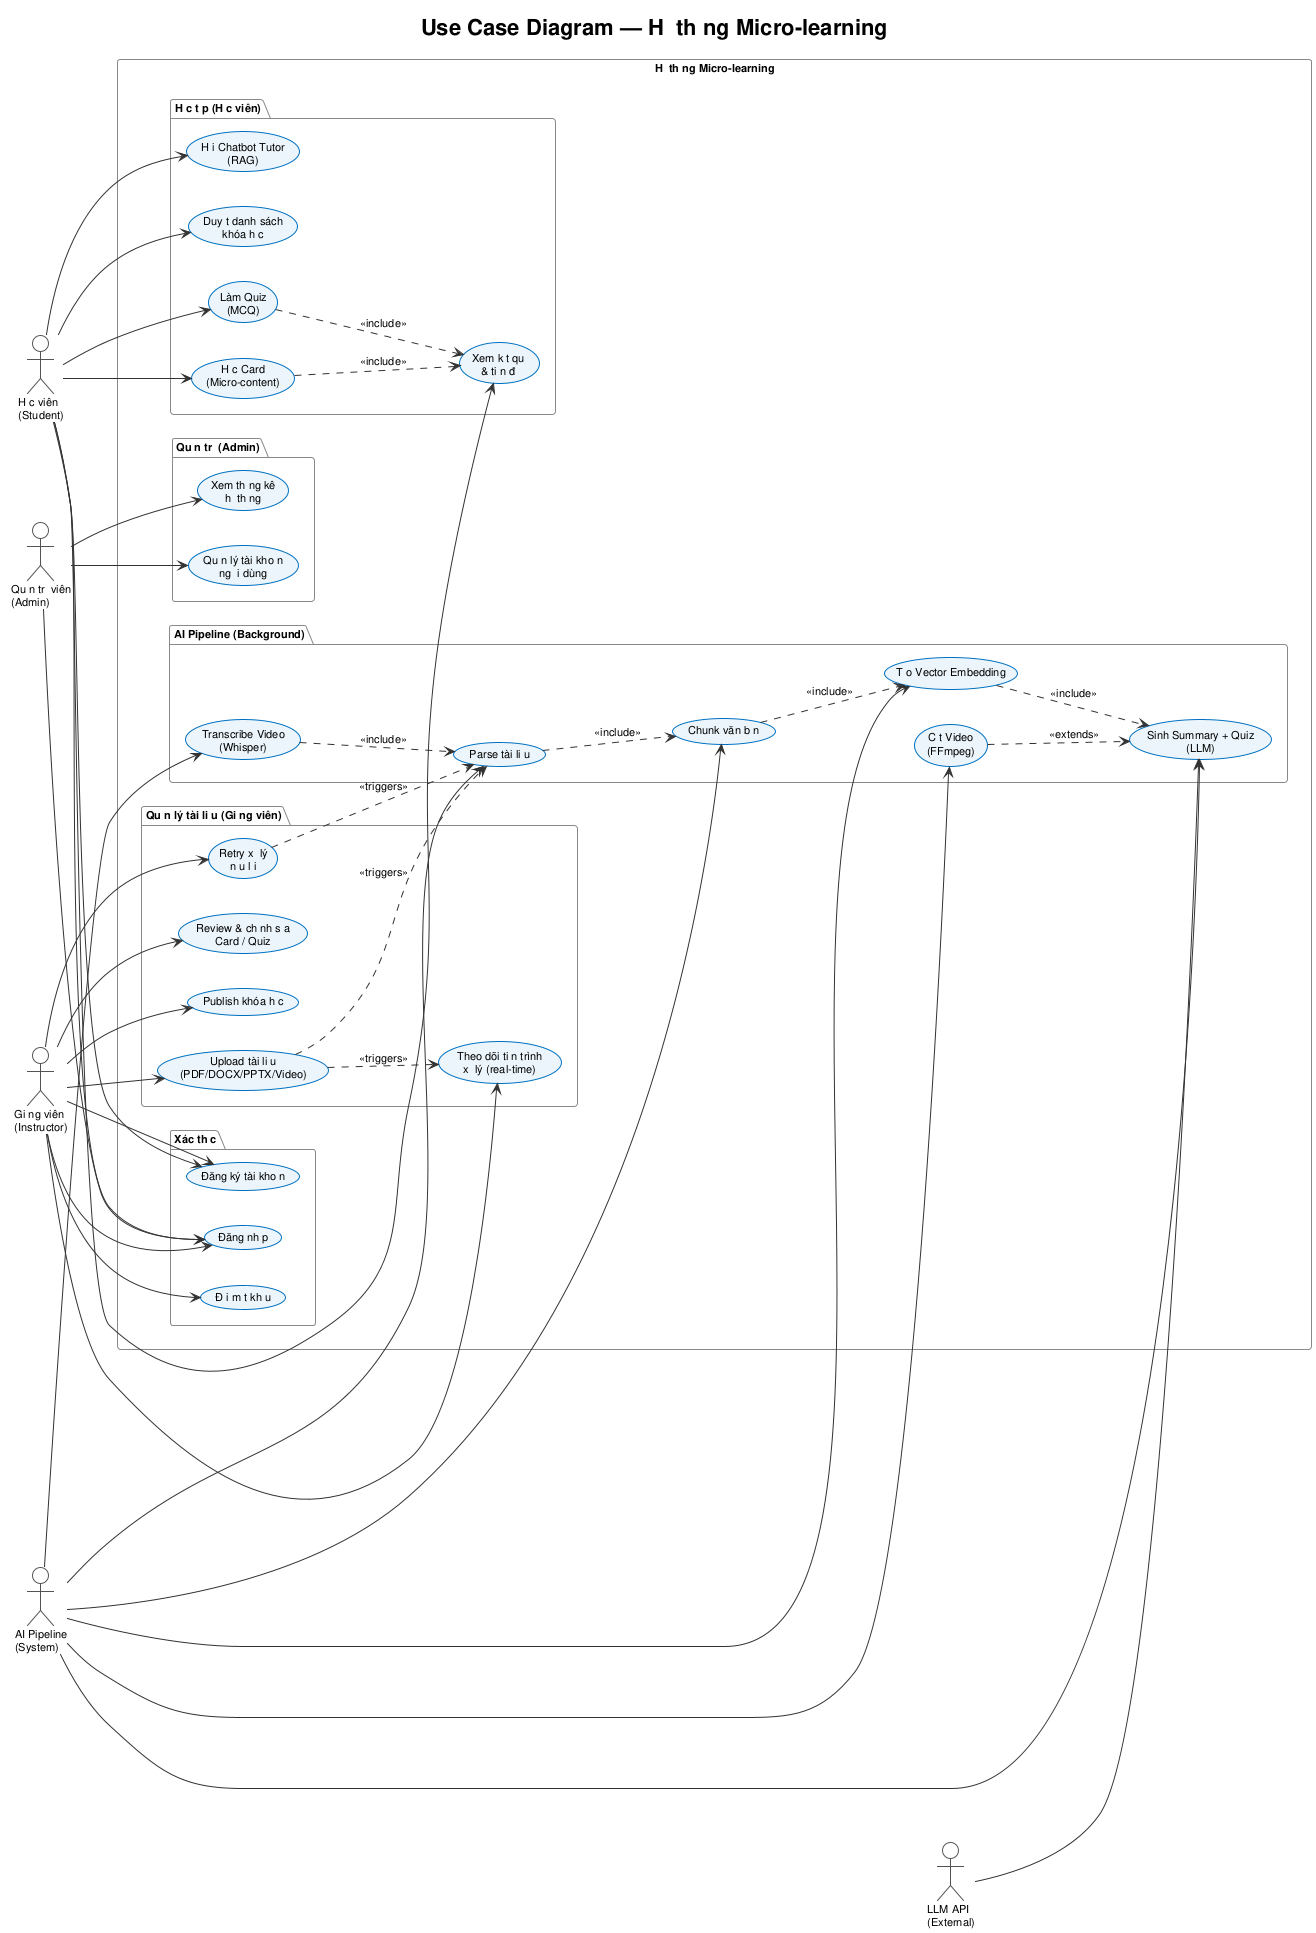
\includegraphics[width=0.88\textwidth,height=0.68\textheight,keepaspectratio]{diagrams/usecase_diagram.png}
    \caption{Use case diagram tổng quát của hệ thống.}
    \label{fig:usecase-diagram-lvtn}
\end{figure}

Các use case chính gồm upload tài liệu, xử lý tài liệu tự động, review nội
dung, publish khóa học, học bằng card, làm quiz, tìm kiếm ngữ nghĩa, ingest
curriculum và quản lý tài khoản. Tác nhân AI Pipeline được mô hình hóa riêng
vì quá trình xử lý diễn ra bất đồng bộ sau khi người dùng upload tài liệu.

\subsection{Đặc tả các Use Case chính}

\subsubsection{UC-01: Upload tài liệu}

\begin{table}[H]
    \centering
    \caption{Thông tin UC-01: Upload tài liệu.}
    \label{tab:uc-upload-lvtn}
    \begin{tabular}{p{3.5cm}p{10.5cm}}
        \toprule
        \textbf{Thuộc tính} & \textbf{Mô tả} \\
        \midrule
        Tác nhân chính & Giảng viên \\
        Tác nhân phụ & AI Pipeline, Object Storage \\
        Mục tiêu & Đưa tài liệu học tập vào hệ thống để bắt đầu pipeline sinh nội dung. \\
        Tiền điều kiện & Giảng viên đã xác thực; khóa học hoặc context LMS đã tồn tại. \\
        Hậu điều kiện & File được lưu, document metadata được tạo, job xử lý được enqueue. \\
        \bottomrule
    \end{tabular}
\end{table}

Luồng chính:
\begin{enumerate}
    \item Giảng viên mở màn hình quản lý tài liệu.
    \item Giảng viên chọn file PDF/DOCX/PPTX và nhập metadata cơ bản.
    \item Frontend kiểm tra định dạng và kích thước.
    \item Backend lưu file vào MinIO và tạo document ở trạng thái
          \texttt{QUEUED}.
    \item Backend enqueue job xử lý tài liệu.
    \item Frontend chuyển sang màn hình theo dõi tiến trình.
\end{enumerate}

Luồng thay thế gồm file sai định dạng, lưu file thất bại hoặc queue tạm thời
không khả dụng. Trong các trường hợp này, hệ thống cần hiển thị lỗi rõ ràng và
cho phép retry khi phù hợp.

\subsubsection{UC-02: Xử lý tài liệu tự động}

\begin{table}[H]
    \centering
    \caption{Thông tin UC-02: Xử lý tài liệu tự động.}
    \label{tab:uc-process-lvtn}
    \begin{tabular}{p{3.5cm}p{10.5cm}}
        \toprule
        \textbf{Thuộc tính} & \textbf{Mô tả} \\
        \midrule
        Tác nhân chính & AI Pipeline \\
        Mục tiêu & Chuyển tài liệu thô thành chunk, embedding, card và quiz. \\
        Tiền điều kiện & File tồn tại trong MinIO; document ở trạng thái \texttt{QUEUED}. \\
        Hậu điều kiện & Document có chunks, vectors, generated cards/quizzes và trạng thái \texttt{DONE}. \\
        \bottomrule
    \end{tabular}
\end{table}

Luồng chính:
\begin{enumerate}
    \item Worker nhận job từ queue.
    \item Worker tải file từ MinIO và chọn parser theo loại file.
    \item Parser trích xuất text, heading và metadata.
    \item Chunker chia tài liệu thành các đơn vị học tập.
    \item Embedder tạo vector và upsert vào Qdrant.
    \item LLM adapter sinh card/quiz cho từng chunk hoặc nhóm chunk.
    \item Metadata store lưu kết quả vào PostgreSQL.
    \item Document chuyển sang \texttt{DONE}.
\end{enumerate}

Luồng thay thế gồm parser lỗi, LLM timeout hoặc Qdrant unavailable. Các lỗi
tạm thời được retry có giới hạn; lỗi cuối cùng được ghi log và chuyển document
sang \texttt{ERROR}.

\subsubsection{UC-03: Review và publish nội dung}

\begin{table}[H]
    \centering
    \caption{Thông tin UC-03: Review và publish nội dung.}
    \label{tab:uc-review-lvtn}
    \begin{tabular}{p{3.5cm}p{10.5cm}}
        \toprule
        \textbf{Thuộc tính} & \textbf{Mô tả} \\
        \midrule
        Tác nhân chính & Giảng viên \\
        Mục tiêu & Kiểm duyệt nội dung do AI sinh ra trước khi học viên truy cập. \\
        Quy tắc nghiệp vụ & Nội dung chưa review không được publish; hệ thống phải lưu dấu vết chỉnh sửa quan trọng. \\
        \bottomrule
    \end{tabular}
\end{table}

Luồng chính:
\begin{enumerate}
    \item Giảng viên mở màn hình review của document đã xử lý.
    \item Hệ thống hiển thị card, quiz, đáp án, giải thích và nguồn chunk.
    \item Giảng viên chỉnh sửa hoặc xóa nội dung chưa phù hợp.
    \item Giảng viên đánh dấu section/document đã review.
    \item Giảng viên publish nội dung cho học viên.
\end{enumerate}

\subsubsection{UC-04: Học bằng card và làm quiz}

\begin{table}[H]
    \centering
    \caption{Thông tin UC-04: Học bằng card và làm quiz.}
    \label{tab:uc-learn-lvtn}
    \begin{tabular}{p{3.5cm}p{10.5cm}}
        \toprule
        \textbf{Thuộc tính} & \textbf{Mô tả} \\
        \midrule
        Tác nhân chính & Học viên \\
        Mục tiêu & Học viên tiếp cận nội dung ngắn, làm câu hỏi kiểm tra và nhận phản hồi. \\
        Dữ liệu lưu & Learning progress, quiz submission, score, timestamp và context bài học. \\
        \bottomrule
    \end{tabular}
\end{table}

Luồng chính:
\begin{enumerate}
    \item Học viên mở bài học từ LMS hoặc trang học tập.
    \item Hệ thống hiển thị danh sách card đã publish.
    \item Học viên đọc card và chuyển sang quiz tương ứng.
    \item Học viên chọn đáp án.
    \item Hệ thống hiển thị đúng/sai, giải thích và lưu kết quả.
\end{enumerate}

\section{Luồng nghiệp vụ chính}

\subsection{Activity Diagrams}

Luồng nghiệp vụ xử lý tài liệu gồm hai nhóm bước chính. Nhóm thứ nhất chuẩn
hóa tri thức từ tài liệu gốc thông qua parse, chunk, embed và persist. Nhóm
thứ hai sinh nội dung học tập thông qua LLM generation, validation và review.
Việc tách hai nhóm bước giúp hệ thống tái sử dụng chunk và embedding cho nhiều
tác vụ khác nhau như search, RAG chatbot hoặc sinh quiz theo Learning Outcome.

\begin{figure}[H]
    \centering
    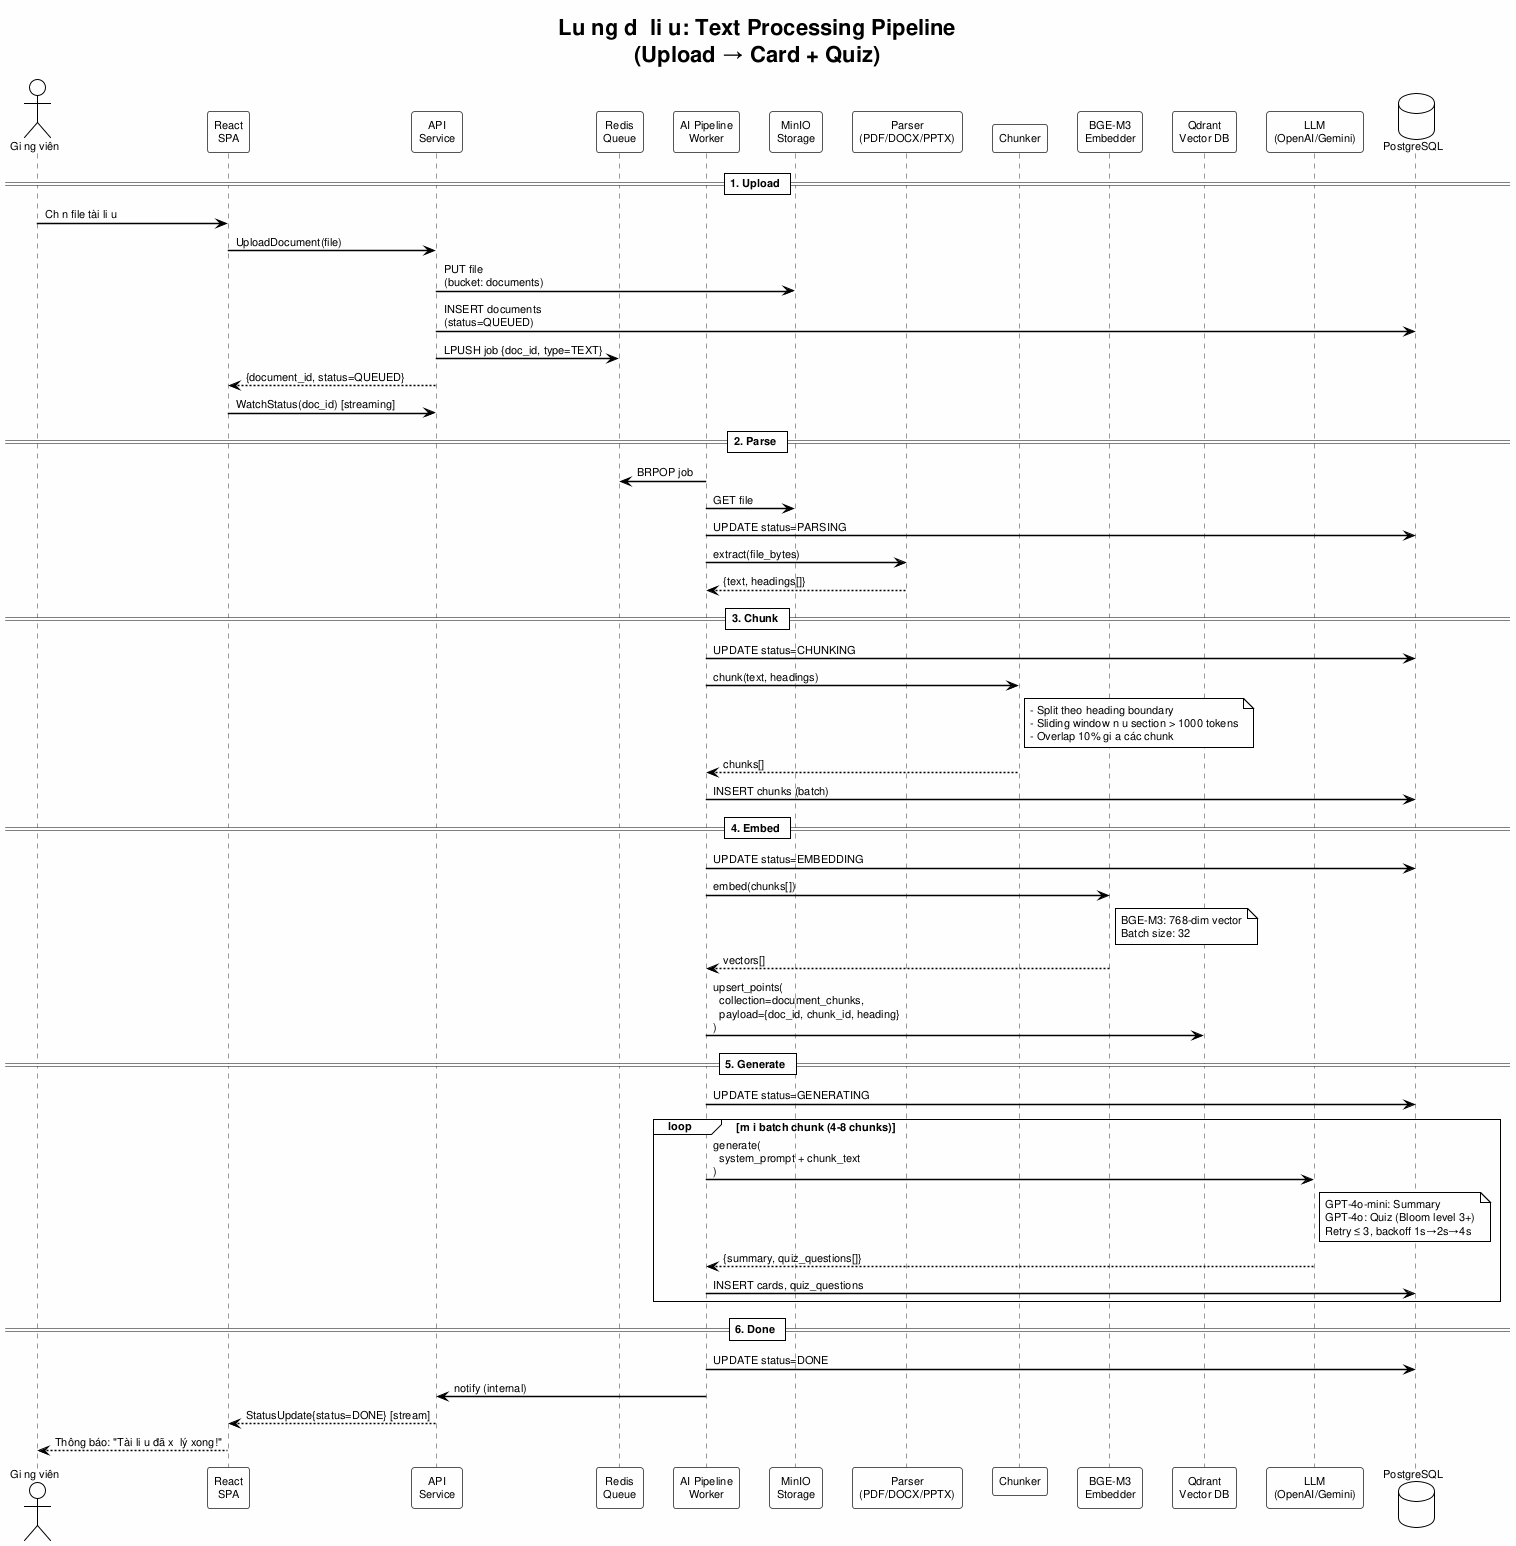
\includegraphics[width=0.92\textwidth]{diagrams/dataflow_text_pipeline.png}
    \caption{Activity/dataflow cho pipeline xử lý tài liệu văn bản.}
    \label{fig:activity-text-pipeline-lvtn}
\end{figure}

\subsection{Dataflow Diagrams}

Luồng RAG bắt đầu từ câu hỏi của học viên hoặc yêu cầu sinh quiz của giảng
viên. Hệ thống tạo embedding cho query, truy xuất chunk liên quan trong
Qdrant, kết hợp metadata và quan hệ trong Knowledge Graph nếu có, sau đó đưa
context vào LLM để sinh câu trả lời hoặc nội dung học tập.

\begin{figure}[H]
    \centering
    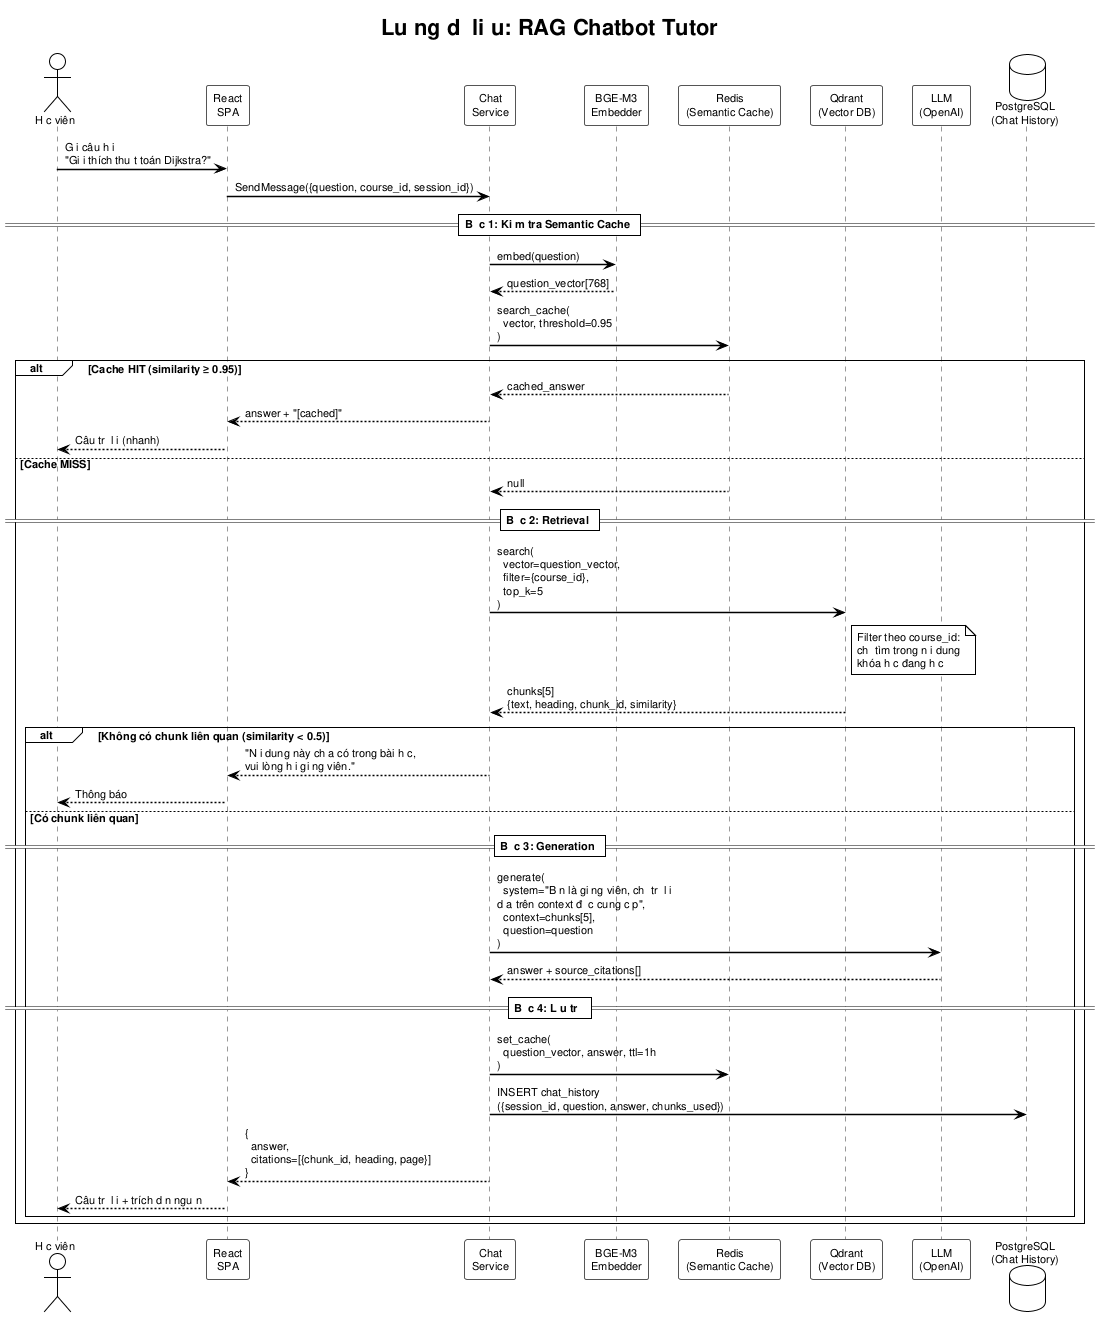
\includegraphics[width=0.92\textwidth]{diagrams/dataflow_rag_chatbot.png}
    \caption{Dataflow cho truy xuất RAG và chatbot học tập.}
    \label{fig:activity-rag-lvtn}
\end{figure}

Các quy tắc nghiệp vụ cần được duy trì trong các luồng trên:
\begin{enumerate}
    \item Học viên chỉ nhìn thấy nội dung đã publish.
    \item Nội dung AI sinh ra phải có nguồn liên kết đến document/chunk gốc.
    \item Quiz sinh theo LO phải lưu LO code, Bloom level và rationale nếu có.
    \item Job xử lý tài liệu phải có trạng thái cuối rõ ràng: \texttt{DONE}
          hoặc \texttt{ERROR}.
    \item Lỗi LLM hoặc vector DB không được làm mất document gốc.
    \item LTI launch phải xác thực trước khi tạo session học tập.
\end{enumerate}


\newpage
\chapter{Thiết kế hệ thống}

\section{Tổng quan kiến trúc hệ thống}

Hệ thống được thiết kế theo hướng tách biệt rõ giữa giao diện người dùng,
logic nghiệp vụ, pipeline AI và hạ tầng lưu trữ. Mục tiêu của kiến trúc là
cho phép thay đổi LLM provider, vector database, graph database hoặc LMS mà
không phải viết lại use case cốt lõi.

\begin{figure}[H]
    \centering
    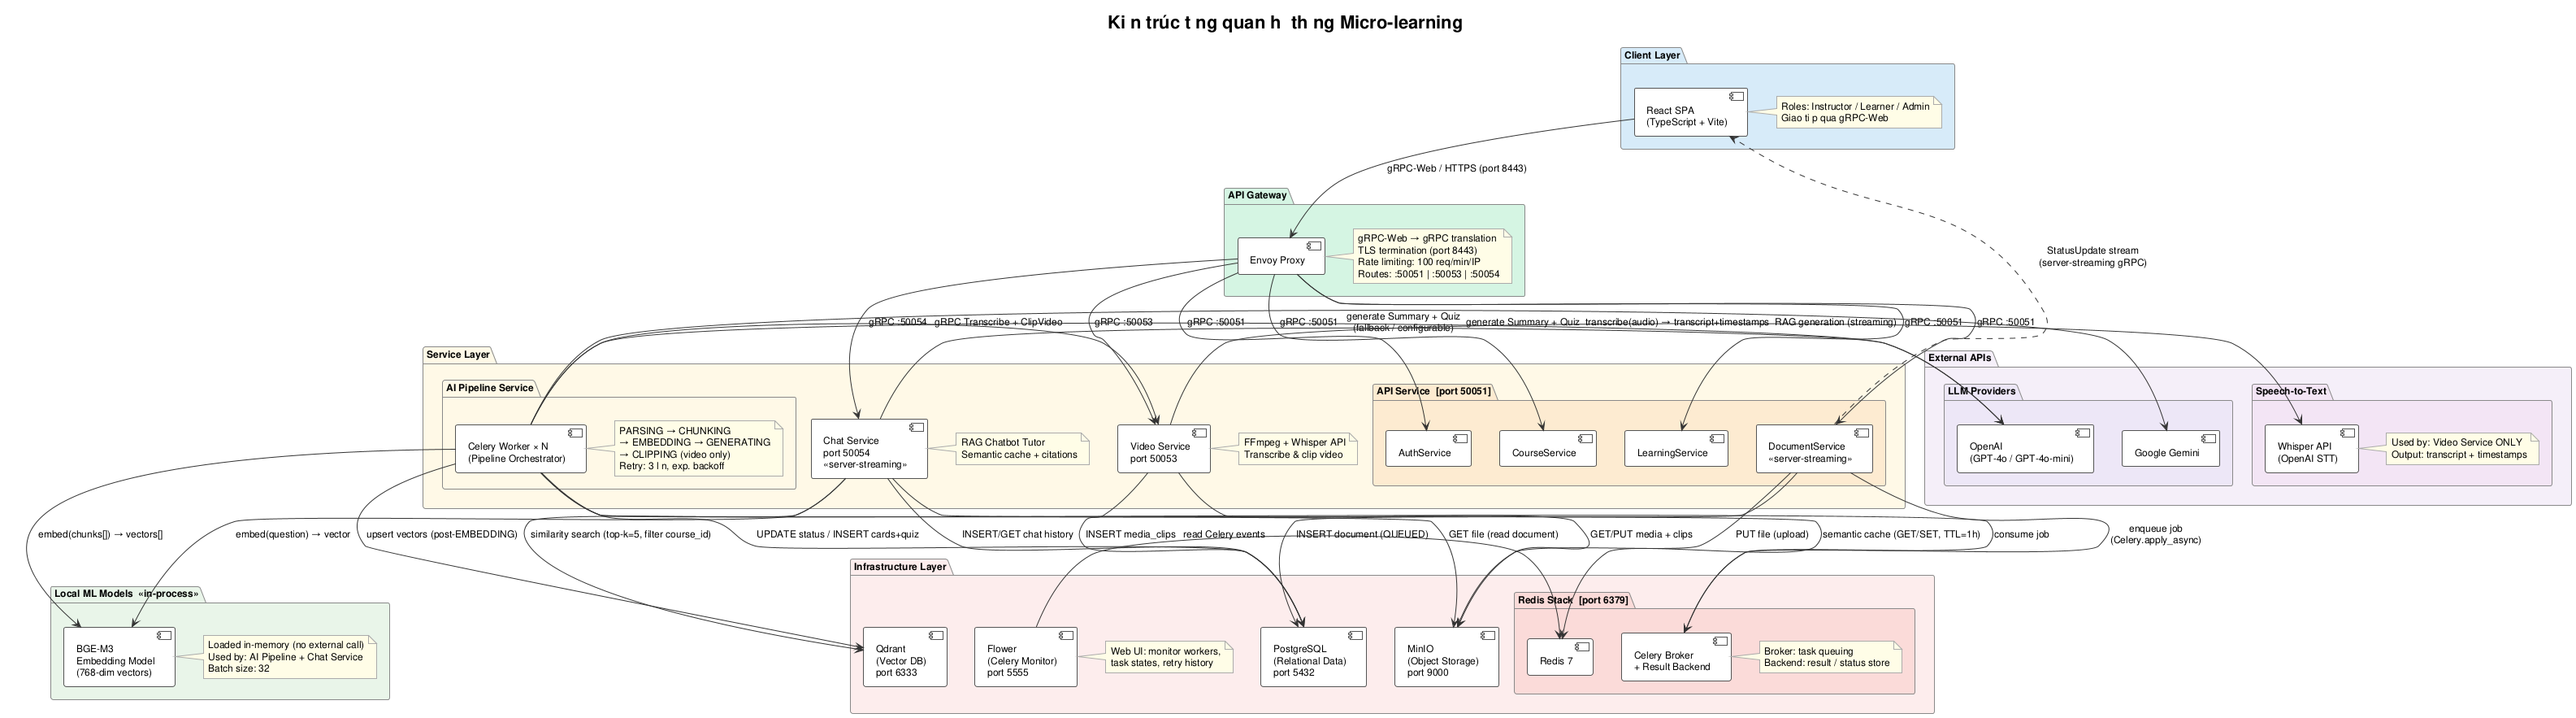
\includegraphics[width=0.95\textwidth]{diagrams/arch_overview.png}
    \caption{Tổng quan kiến trúc hệ thống.}
    \label{fig:arch-overview-lvtn}
\end{figure}

Các lớp chính trong hệ thống gồm:
\begin{itemize}
    \item \textbf{LMS layer:} Open edX hoặc Moodle đóng vai trò nền tảng học
          tập chính, gọi hệ thống qua LTI 1.3.
    \item \textbf{Frontend layer:} Next.js cung cấp màn hình review cho giảng
          viên, màn hình học cho học viên và route xử lý LTI.
    \item \textbf{Application/API layer:} Python gRPC service expose các use
          case như upload/process/search/get quiz/ingest curriculum.
    \item \textbf{Worker layer:} document worker, enrichment worker và outbox
          worker xử lý bất đồng bộ.
    \item \textbf{Storage layer:} PostgreSQL lưu metadata, MinIO lưu file,
          Qdrant lưu vector, Neo4j lưu Knowledge Graph.
    \item \textbf{AI provider layer:} LLM và embedding model được gọi qua
          adapter để giảm phụ thuộc vào provider cụ thể.
\end{itemize}

Backend AI áp dụng Hexagonal Architecture. Domain/application layer chứa các
entity và use case cốt lõi; ports định nghĩa interface cho parser, chunker,
embedder, vector store, graph store, metadata store và LLM client; adapters
hiện thực giao tiếp với PostgreSQL, Qdrant, Neo4j, MinIO, Redis và provider
AI.

\begin{figure}[H]
    \centering
    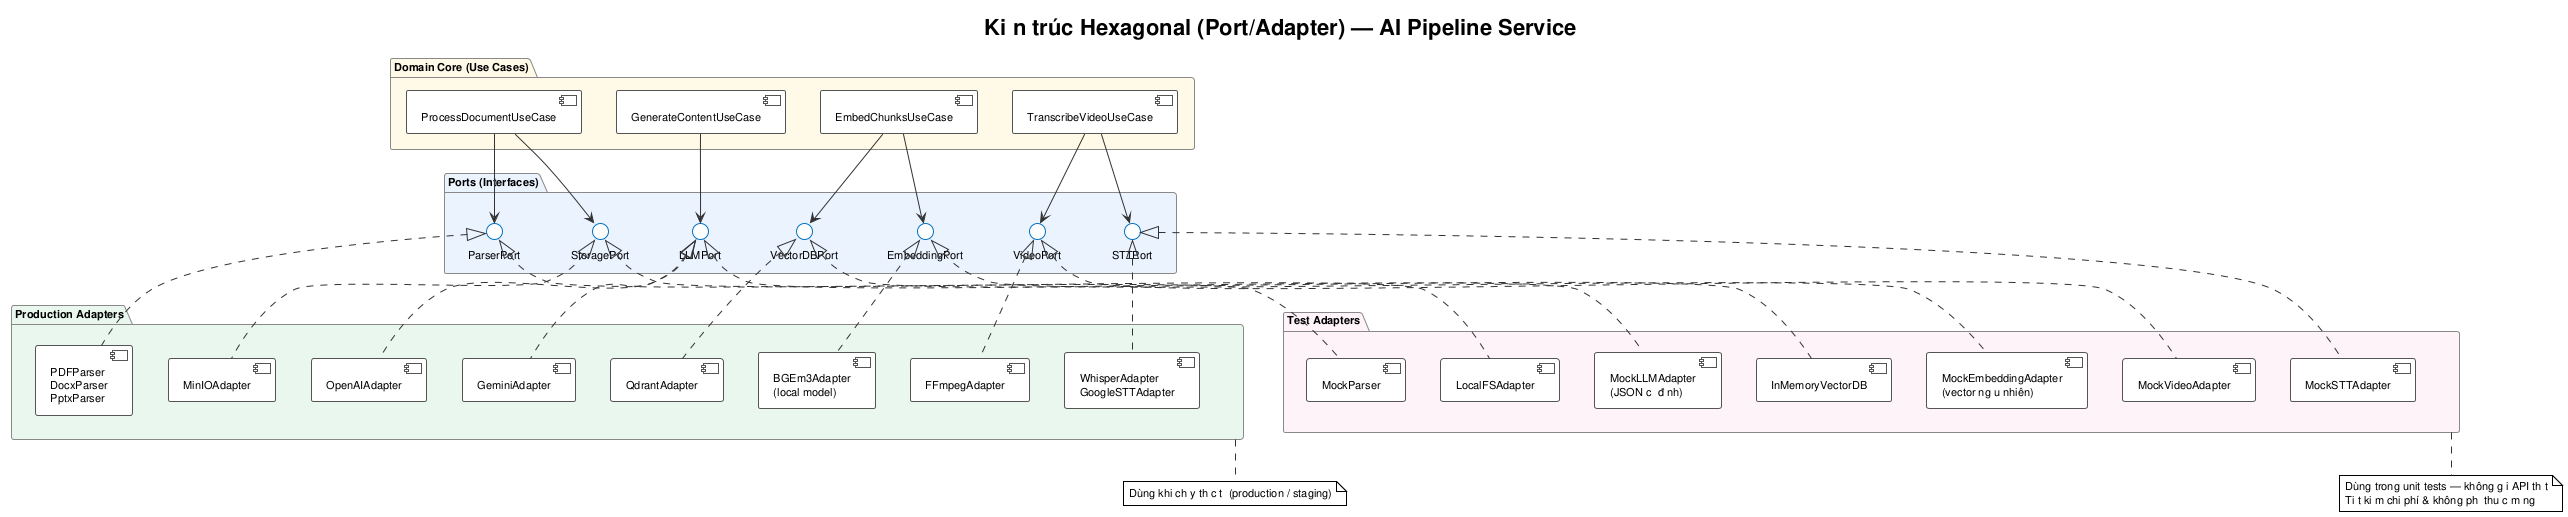
\includegraphics[width=0.95\textwidth]{diagrams/arch_hexagonal.png}
    \caption{Kiến trúc Hexagonal trong backend AI.}
    \label{fig:hexagonal-lvtn}
\end{figure}

\section{Kiến trúc tích hợp LMS}

\subsection{Open edX / Moodle}

Open edX là nền tảng tích hợp chính trong phạm vi hiện tại. Hệ thống được
nhúng vào khóa học thông qua LTI 1.3. Khi học viên hoặc giảng viên mở activity
từ Open edX, LMS gửi LTI launch request đến frontend. Frontend xác thực
request, tạo session và điều hướng đến màn hình phù hợp với vai trò người
dùng.

Moodle được phân tích như hướng triển khai tương thích. Vì hệ thống đóng vai
trò LTI Tool Provider, về nguyên tắc có thể đăng ký như external tool trong
Moodle mà không cần thay đổi lõi backend. Sự khác biệt chủ yếu nằm ở cấu hình
platform, deployment ID, client ID, keyset URL và mapping role/context.

\subsection{LTI 1.3 Flow}

\begin{figure}[H]
    \centering
    
\includegraphics[width=0.95\textwidth]{figures/lti_auth_flow.png}
    \caption{Luồng xác thực LTI 1.3/OIDC.}
    \label{fig:lti-flow-lvtn}
\end{figure}

Hệ thống hoạt động như LTI Tool. Khi người dùng click từ LMS, LMS khởi tạo
OIDC login, sau đó gửi LTI launch request chứa JWT đã ký. Frontend/route LTI
kiểm tra issuer, client ID, deployment ID, nonce, signature và claim người
dùng. Sau khi xác thực, hệ thống tạo session nội bộ và điều hướng người dùng
đến màn hình tương ứng.

\subsection{Vai trò LMS trong hệ thống}

LMS giữ vai trò quản lý khóa học, danh sách người dùng, phân quyền ban đầu và
điểm truy cập học tập. Hệ thống AI không thay thế LMS mà bổ sung một tool bên
ngoài để tạo và phân phối Micro-Content/Quiz. Thiết kế này giúp giảm rủi ro
triển khai vì cơ sở đào tạo vẫn có thể giữ quy trình LMS hiện hữu.

\section{Thiết kế AI Pipeline}

\subsection{Trích xuất tài liệu}

Sau khi giảng viên upload file, backend lưu file gốc vào MinIO và tạo metadata
document trong PostgreSQL. Worker nhận job từ queue, tải file và chọn parser
theo định dạng. Parser trích xuất text, heading, page range và metadata cần
thiết để phục vụ chunking và truy xuất nguồn về sau.

\subsection{OCR}

OCR được đặt sau bước phát hiện text layer. Nếu PDF có text layer đủ chất
lượng, hệ thống đọc trực tiếp văn bản. Nếu PDF là ảnh hoặc lượng text trích
xuất quá ít, pipeline chuyển sang OCR. Kết quả OCR cần lưu confidence để
giảng viên biết phần nào có nguy cơ sai khi review.

Trong phạm vi hiện tại, OCR production cho tài liệu scan chất lượng thấp được
xem là thiết kế mở rộng. Pipeline vẫn chừa adapter OCR để có thể bổ sung
Tesseract hoặc dịch vụ OCR chuyên biệt khi cần.

\subsection{Chunking}

Chunking chia tài liệu dài thành các đơn vị đủ nhỏ để embedding và đưa vào
prompt, nhưng vẫn đủ ngữ cảnh để giữ ý nghĩa học thuật. Hệ thống ưu tiên
heading-based chunking cho tài liệu có cấu trúc rõ. Mỗi chunk giữ heading path
như ``Chương 2 > 2.1 Khái niệm'', page range và document ID.

Với tài liệu thiếu heading, hệ thống dùng fallback chunking theo kích thước
token/ký tự và overlap. Overlap giúp giảm rủi ro cắt mất thông tin giữa hai
chunk liên tiếp nhưng cần được cấu hình hợp lý để tránh tăng chi phí embedding
và LLM.

\subsection{Embedding}

Mỗi chunk sau khi tạo được chuyển thành embedding bằng mô hình đa ngôn ngữ.
Vector được lưu vào Qdrant cùng payload metadata như course ID, document ID,
chunk ID, heading path, language và page range. Metadata này cho phép hệ thống
lọc retrieval theo khóa học, tài liệu hoặc chương.

\subsection{Retrieval}

Retrieval được dùng cho semantic search, RAG chatbot và sinh quiz theo LO.
Luồng truy xuất gồm embed query, tìm top-K chunk trong Qdrant, lọc theo
metadata và tăng ưu tiên bằng quan hệ Knowledge Graph nếu có. Với LMS, bước
lọc theo course/context là bắt buộc để tránh truy xuất nhầm nội dung ngoài
quyền truy cập của người học.

\subsection{Generation}

LLM generation nhận prompt gồm instruction, context chunk, Learning Outcome,
Bloom level, số lượng câu hỏi và schema đầu ra. Nội dung sinh ra được validate
theo JSON schema, rule nghiệp vụ và liên kết nguồn. Kết quả hợp lệ được lưu
như bản nháp để giảng viên review; hệ thống không publish tự động nội dung do
AI sinh ra.

\section{Thiết kế lưu trữ và dữ liệu}

\subsection{PostgreSQL}

PostgreSQL là source of truth cho dữ liệu nghiệp vụ. Các nhóm bảng chính gồm:
\begin{itemize}
    \item \textbf{Document:} document, file metadata, trạng thái pipeline.
    \item \textbf{Chunking:} chunk content, heading path, vị trí trong tài
          liệu, metadata ngôn ngữ.
    \item \textbf{Generated content:} lesson card, quiz item, đáp án, giải
          thích, trạng thái review.
    \item \textbf{Curriculum:} course, chapter, learning outcome, assessment,
          mapping LO-assessment và chunk-LO.
    \item \textbf{Learning data:} progress, quiz submission, score và event
          học tập.
\end{itemize}

\begin{figure}[H]
    \centering
    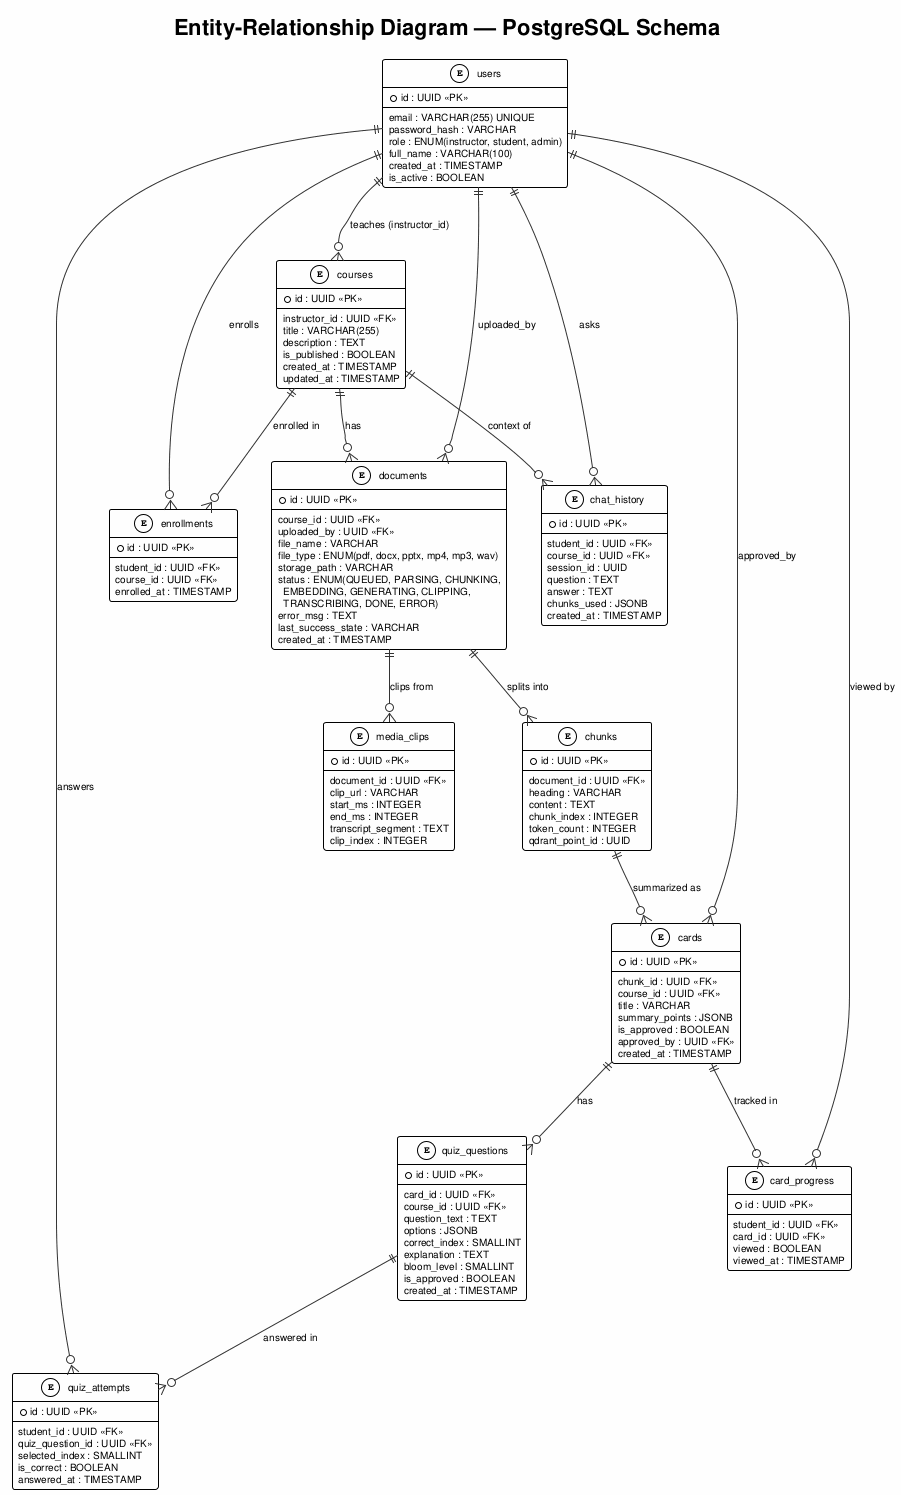
\includegraphics[width=0.95\textwidth,height=0.78\textheight,keepaspectratio]{diagrams/er_diagram.png}
    \caption{ER diagram của hệ thống.}
    \label{fig:er-lvtn}
\end{figure}

\subsection{Qdrant Vector DB}

Qdrant lưu vector embedding của chunk và payload metadata. Mỗi vector point
đại diện cho một chunk. Các thao tác chính gồm tạo collection theo kích thước
embedding, upsert vector sau khi chunking, search top-K theo query vector và
filter theo course, document hoặc language.

\subsection{Neo4j Graph DB}

Neo4j lưu projection Knowledge Graph cho curriculum. PostgreSQL vẫn giữ dữ
liệu gốc, còn Neo4j tối ưu cho truy vấn quan hệ tri thức như chunk nào hỗ trợ
LO nào, assessment nào đo LO nào hoặc chapter nào liên quan đến một nhóm
chuẩn đầu ra.

\subsection{MinIO / Object Storage}

MinIO lưu file gốc được upload bởi giảng viên. Metadata trong PostgreSQL chỉ
lưu đường dẫn object, checksum, MIME type, kích thước và trạng thái xử lý. Cách
tách này giúp database không phải lưu binary lớn và cho phép worker tải file
theo nhu cầu.

\subsection{Redis / Queue}

Redis và queue được dùng cho các job bất đồng bộ như parse document, sinh
embedding, gọi LLM và đồng bộ graph. Mỗi job cần lưu trạng thái, số lần retry,
thời điểm bắt đầu/kết thúc và lỗi cuối cùng để frontend có thể hiển thị tiến
trình cho giảng viên.

\section{Thiết kế mô hình tri thức và chiến lược truy xuất}

\subsection{Curriculum-aware Retrieval}

Curriculum-aware retrieval đưa thông tin chương trình học vào quá trình chọn
context. Khi giảng viên chọn một Learning Outcome hoặc chapter, hệ thống ưu
tiên chunk có quan hệ trực tiếp với LO/chapter đó trước khi đưa vào prompt.
Cách làm này giúp quiz bám mục tiêu học tập hơn so với chỉ dựa trên vector
similarity.

\subsection{GraphRAG Strategies}

GraphRAG trong luận văn được thiết kế theo ba mức:
\begin{enumerate}
    \item \textbf{Graph filtering:} chỉ lấy chunk có quan hệ với LO/chapter
          mục tiêu.
    \item \textbf{Graph-aware reranking:} kết hợp điểm vector similarity với
          điểm quan hệ trong graph.
    \item \textbf{Graph explanation:} lưu rationale để giải thích vì sao một
          chunk hoặc quiz liên quan đến LO.
\end{enumerate}

Reasoning đa bước trên graph được xem là hướng mở rộng, không trình bày như
kết quả hoàn thiện trong giai đoạn hiện tại.

\subsection{Metadata Strategy}

Metadata được lưu nhất quán giữa PostgreSQL, Qdrant và Neo4j. Các khóa quan
trọng gồm \texttt{course\_id}, \texttt{document\_id}, \texttt{chunk\_id},
\texttt{chapter\_id}, \texttt{lo\_id}, heading path, page range, language và
source version. Metadata giúp truy xuất có thể lọc theo phạm vi khóa học,
truy ngược nguồn và đánh giá chất lượng retrieval.

\subsection{Knowledge Graph Structure}

Các node chính của Knowledge Graph gồm Course, Chapter, LearningOutcome,
Assessment và Chunk. Các quan hệ chính gồm:
\begin{itemize}
    \item \texttt{COURSE\_HAS\_CHAPTER}: Course chứa Chapter.
    \item \texttt{CHAPTER\_HAS\_LO}: Chapter chứa hoặc liên quan đến LO.
    \item \texttt{ASSESSMENT\_MEASURES\_LO}: Assessment đo LO.
    \item \texttt{CHUNK\_SUPPORTS\_LO}: Chunk hỗ trợ đạt LO.
\end{itemize}

Knowledge Graph được dùng cho ba mục tiêu: truy xuất chunk theo LO, giải
thích liên kết giữa quiz và chuẩn đầu ra, và chuẩn bị nền tảng cho adaptive
learning hoặc GraphRAG nâng cao.

\section{Giao tiếp và tích hợp hệ thống}

\subsection{gRPC API}

Backend expose gRPC API cho các use case chính. gRPC được chọn cho giao tiếp
nội bộ vì contract rõ ràng, sinh mã client/server thuận tiện và phù hợp giữa
frontend/API gateway, backend AI service và worker runner.

\begin{figure}[H]
    \centering
    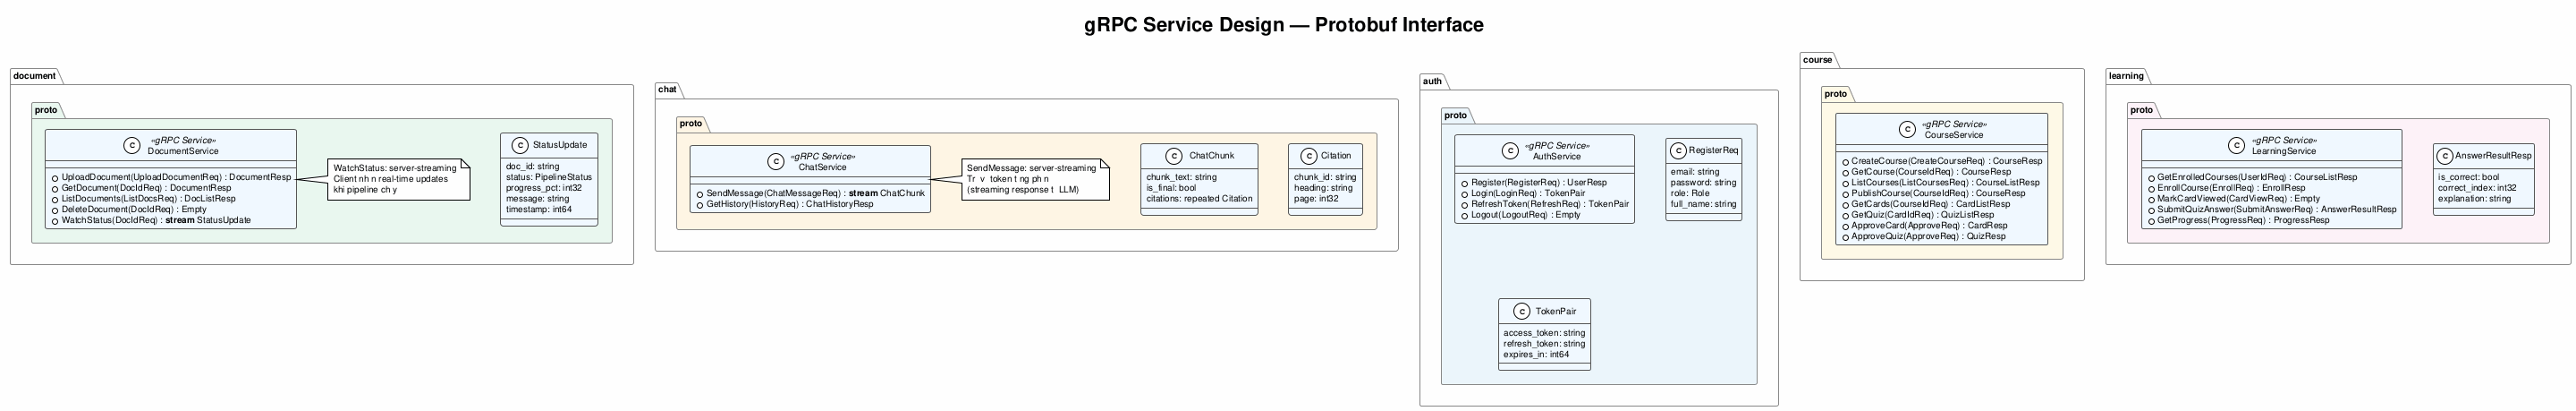
\includegraphics[width=0.95\textwidth]{diagrams/grpc_service_design.png}
    \caption{Thiết kế gRPC service và các use case tương ứng.}
    \label{fig:grpc-design-lvtn}
\end{figure}

\subsection{Internal Services}

Các nhóm service chính trong hệ thống gồm:
\begin{table}[H]
    \centering
    \caption{Các service chính trong kiến trúc triển khai.}
    \label{tab:services-lvtn}
    \begin{tabular}{p{3.5cm}p{10.5cm}}
        \toprule
        \textbf{Service} & \textbf{Vai trò} \\
        \midrule
        Next.js frontend & UI, LTI login/launch, proxy hoặc gọi API backend. \\
        Python gRPC service & API xử lý tài liệu, search, curriculum và quiz. \\
        Document worker & Parse, chunk, embed và lưu kết quả xử lý tài liệu. \\
        Enrichment worker & Sinh card/quiz bằng LLM và validate kết quả. \\
        Outbox worker & Đồng bộ sự kiện từ PostgreSQL sang Neo4j. \\
        PostgreSQL & Source of truth cho metadata, document, chunk, card, quiz và curriculum. \\
        Qdrant & Vector store phục vụ semantic search và retrieval. \\
        Neo4j & Knowledge Graph cho Course, Chapter, LO, Assessment và quan hệ SUPPORTS. \\
        MinIO & Object storage cho file gốc. \\
        Redis/Queue & Queue và trạng thái xử lý bất đồng bộ. \\
        \bottomrule
    \end{tabular}
\end{table}

\subsection{Async Workers}

Worker giúp tách tác vụ nặng khỏi request/response trực tiếp. Document worker
xử lý parse, chunk và embed; enrichment worker sinh nội dung học tập; outbox
worker đồng bộ dữ liệu sang graph. Các worker đọc job từ queue, cập nhật trạng
thái document và ghi log lỗi để người dùng có thể retry khi cần.

\subsection{Event / Queue Flow}

Sau khi upload thành công, backend tạo document ở trạng thái \texttt{QUEUED}
và enqueue job. Worker chuyển trạng thái qua các bước \texttt{PARSING},
\texttt{CHUNKING}, \texttt{EMBEDDING}, \texttt{GENERATING}, sau đó kết thúc
bằng \texttt{DONE} hoặc \texttt{ERROR}. Các sự kiện liên quan đến curriculum
và chunk-LO mapping được ghi vào outbox để đồng bộ sang Neo4j.

\section{Sequence Diagrams và System Flows}

\subsection{Luồng ingest curriculum}

\begin{figure}[H]
    \centering
    
\includegraphics[width=0.95\textwidth]{figures/seq_ingest_curriculum.png}
    \caption{Sequence diagram cho luồng ingest đề cương môn học.}
    \label{fig:seq-ingest-curriculum-lvtn}
\end{figure}

Luồng ingest curriculum bắt đầu từ request của giảng viên hoặc admin, sau đó
backend gọi parser để trích xuất Course, Chapter, Learning Outcome và
Assessment. Dữ liệu được lưu vào PostgreSQL trước, sau đó outbox/event
projector đồng bộ sang Neo4j. Thiết kế này giữ PostgreSQL làm source of truth
và cho phép Neo4j được rebuild nếu cần.

\subsection{Luồng xử lý tài liệu}

Luồng xử lý tài liệu gồm các bước upload, enqueue, parse, chunk, embed,
generate và persist. Các bước có thể retry độc lập ở cấp job. Trạng thái
document được cập nhật để frontend có thể hiển thị tiến trình cho giảng viên.

\begin{table}[H]
    \centering
    \caption{Trạng thái pipeline xử lý tài liệu.}
    \label{tab:pipeline-states-lvtn}
    \begin{tabular}{p{3cm}p{10.5cm}}
        \toprule
        \textbf{Trạng thái} & \textbf{Ý nghĩa} \\
        \midrule
        \texttt{QUEUED} & Document đã lưu và đang chờ worker xử lý. \\
        \texttt{PARSING} & Worker đang trích xuất text/metadata từ file. \\
        \texttt{CHUNKING} & Nội dung đang được chia thành chunk học tập. \\
        \texttt{EMBEDDING} & Chunk đang được chuyển thành vector. \\
        \texttt{GENERATING} & LLM đang sinh card/quiz. \\
        \texttt{DONE} & Pipeline hoàn tất thành công. \\
        \texttt{ERROR} & Pipeline thất bại sau số lần retry cho phép. \\
        \bottomrule
    \end{tabular}
\end{table}

\subsection{Luồng học và làm quiz}

Khi học viên mở tool từ LMS, hệ thống xác thực LTI launch và tạo session. Học
viên chỉ nhìn thấy nội dung đã publish. Khi làm quiz, submission được lưu cùng
score, đáp án đã chọn, thời điểm làm bài và context bài học. Dữ liệu này là
nền tảng cho dashboard học tập và recommendation/adaptive learning trong giai
đoạn sau.


\newpage
\chapter{Hiện thực và triển khai}

\section{Môi trường và công cụ phát triển}

Hệ thống được hiện thực thành nhiều thành phần chạy trong Docker Compose:
frontend Next.js, backend Python gRPC, các worker xử lý bất đồng bộ và các
dịch vụ hạ tầng gồm PostgreSQL, Redis, MinIO, Qdrant và Neo4j. Cách triển
khai này phù hợp cho môi trường phát triển, demo và staging; khi đưa vào
production có thể chuyển dần sang Kubernetes.

Các công cụ chính gồm:
\begin{itemize}
    \item \textbf{Next.js/TypeScript:} xây dựng giao diện người dùng và route
          LTI.
    \item \textbf{Python gRPC services:} hiện thực API và use case AI.
    \item \textbf{PostgreSQL, Qdrant, Neo4j, MinIO, Redis:} các thành phần lưu
          trữ và queue.
    \item \textbf{Docker Compose:} tái lập môi trường chạy local/staging.
    \item \textbf{LLM/Embedding provider:} sinh nội dung, embedding và hỗ trợ
          structured output.
\end{itemize}

\begin{figure}[H]
    \centering
    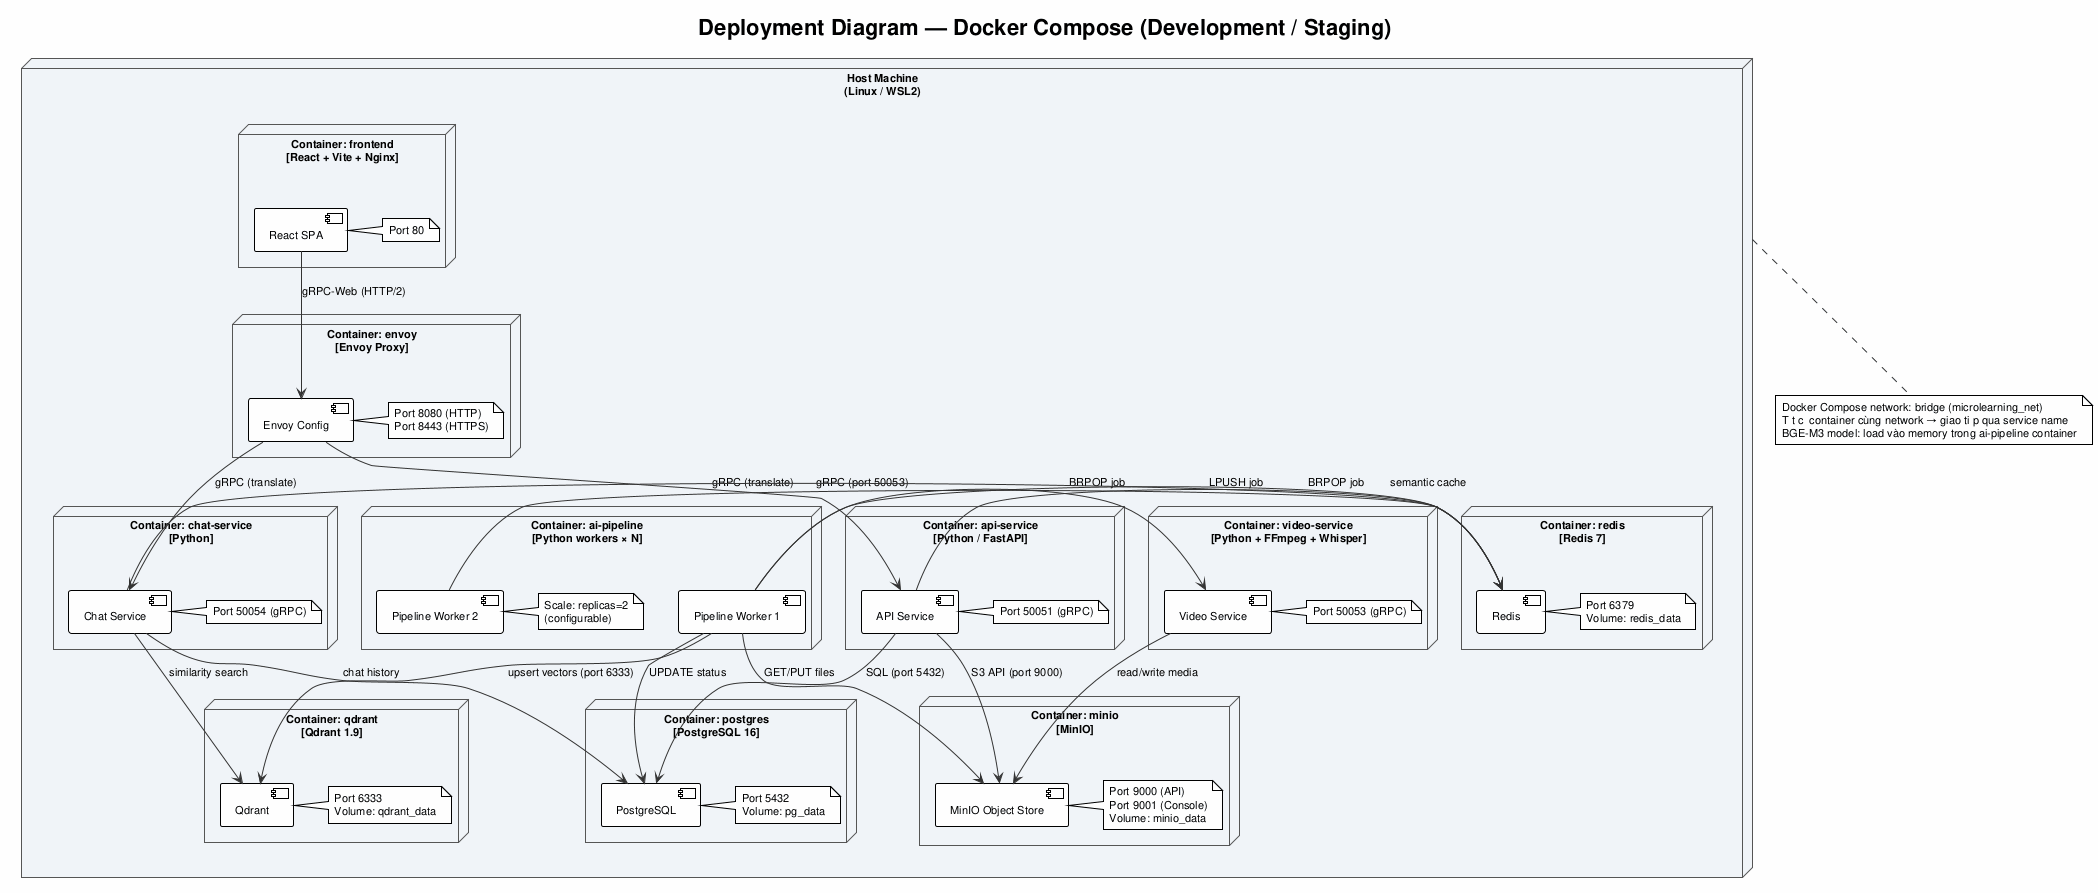
\includegraphics[width=0.95\textwidth]{diagrams/deployment_diagram.png}
    \caption{Deployment diagram của hệ thống.}
    \label{fig:deployment-implementation-lvtn}
\end{figure}

\section{Hiện thực Frontend và Backend}

\subsection{Next.js}

Frontend được xây dựng bằng Next.js và TypeScript. Thành phần này đảm nhận ba
vai trò chính:
\begin{itemize}
    \item Cung cấp giao diện giảng viên để upload, review và quản lý nội dung.
    \item Cung cấp giao diện học viên để xem card, làm quiz và nhận phản hồi.
    \item Xử lý LTI login/launch route để tích hợp với LMS.
\end{itemize}

Cấu trúc route chính:
\begin{itemize}
    \item \texttt{/lti/login}: khởi tạo OIDC login flow.
    \item \texttt{/lti/launch}: nhận LTI launch request và tạo session.
    \item \texttt{/manage/review}: màn hình giảng viên review nội dung AI.
    \item \texttt{/learn/cards}: màn hình học card.
    \item \texttt{/learn/quiz/[documentId]}: màn hình làm quiz theo tài liệu.
\end{itemize}

Session LTI được lưu phía server để giảm rủi ro lộ claim nhạy cảm trên client.
Frontend không tự quyết định quyền truy cập quan trọng mà dựa trên context đã
xác thực từ LTI/session và backend.

\subsection{Python gRPC Services}

Backend AI được hiện thực bằng Python, tổ chức theo Hexagonal Architecture.
Các use case chính nằm ở application layer, được gọi từ gRPC delivery hoặc
worker runner.

\begin{figure}[H]
    \centering
    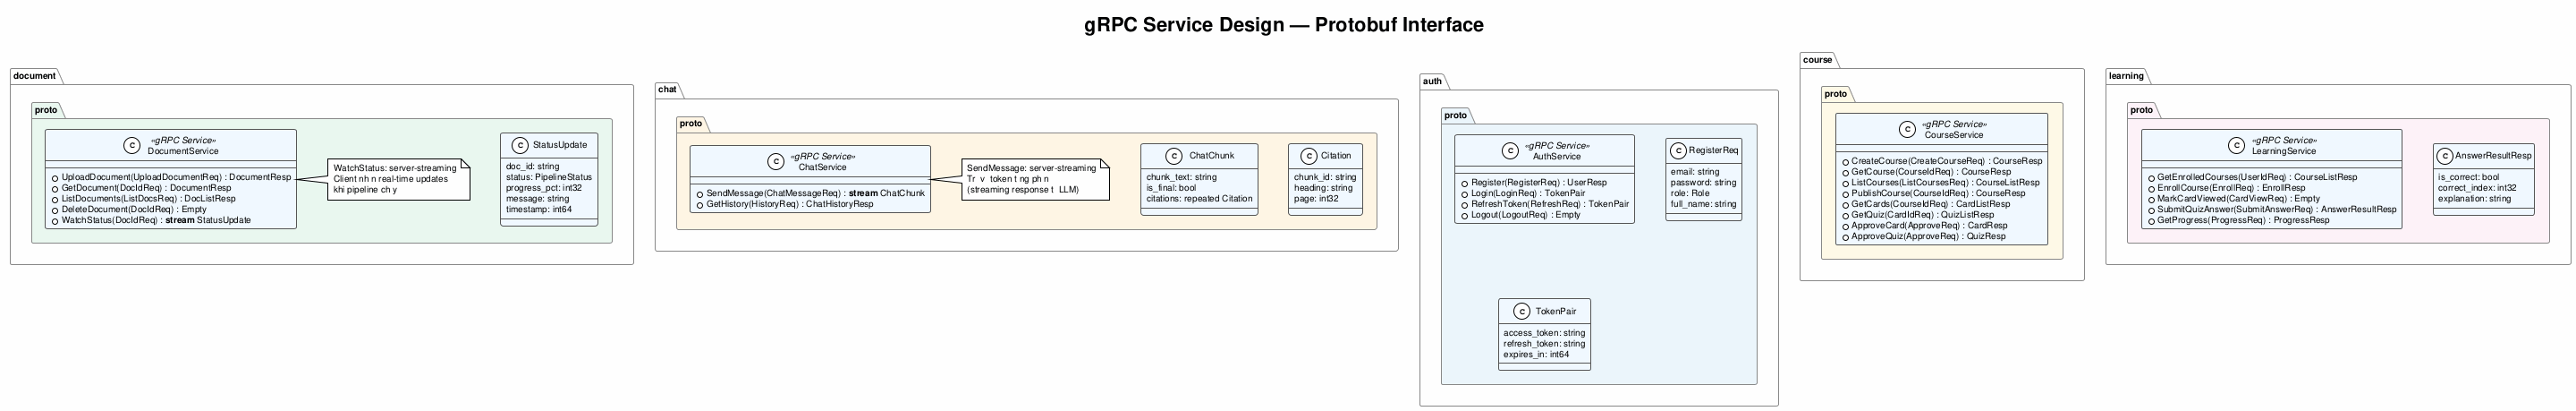
\includegraphics[width=0.95\textwidth]{diagrams/grpc_service_design.png}
    \caption{Hiện thực gRPC service và các use case tương ứng.}
    \label{fig:grpc-implementation-lvtn}
\end{figure}

Các nhóm API/use case chính:
\begin{itemize}
    \item \textbf{Document:} enqueue, process, delete, get status.
    \item \textbf{Search:} search chunks, search by learning outcome.
    \item \textbf{Generated content:} get cards, get quiz, generate curriculum
          quiz.
    \item \textbf{Curriculum:} ingest curriculum, list LO/chapter/assessment.
\end{itemize}

Dependency injection container khởi tạo adapter theo cấu hình môi trường. Khi
thiếu một dịch vụ hạ tầng trong môi trường test, hệ thống có thể dùng adapter
noop hoặc mock để kiểm thử use case.

\subsection{API Gateway}

API Gateway hoặc frontend server đóng vai trò cầu nối giữa UI, LTI session và
backend gRPC. Thành phần này kiểm tra session, chuyển đổi request từ giao diện
sang contract backend và mapping lỗi kỹ thuật thành thông báo dễ hiểu cho
người dùng. Với các endpoint cần streaming hoặc xử lý lâu, gateway chỉ khởi
tạo job và trả về trạng thái để frontend polling hoặc subscribe tiến trình.

\section{Hiện thực luồng xử lý bất đồng bộ}

\subsection{Workers}

Các worker giúp tách tác vụ nặng khỏi request/response trực tiếp:
\begin{itemize}
    \item \textbf{Document worker:} nhận job tài liệu, parse, chunk, embed và
          lưu metadata.
    \item \textbf{Enrichment worker:} sinh card/quiz bằng LLM và validate kết
          quả.
    \item \textbf{Outbox worker:} đọc sự kiện hoặc bảng outbox từ PostgreSQL
          để đồng bộ sang Neo4j.
\end{itemize}

Mô hình worker giúp frontend phản hồi nhanh sau khi upload, còn xử lý tài liệu
diễn ra bất đồng bộ. Khi lỗi tạm thời xảy ra, job có thể retry mà không yêu
cầu người dùng upload lại file.

\subsection{Queue}

Queue lưu các job xử lý tài liệu, embedding và generation. Mỗi job cần có
document ID, course context, số lần retry, trạng thái hiện tại và thông tin lỗi
cuối cùng. Worker cập nhật trạng thái để frontend hiển thị tiến trình cho
giảng viên.

\subsection{Embedding Jobs}

Embedding job nhận danh sách chunk đã được parse/chunk thành công. Worker gọi
embedding provider, chuẩn hóa vector và upsert vào Qdrant cùng metadata. Nếu
Qdrant hoặc provider tạm thời lỗi, job được retry có giới hạn; nếu hết retry,
document chuyển sang trạng thái lỗi để người dùng có thể xử lý lại.

\subsection{Quiz Generation Jobs}

Quiz generation job nhận context chunk, Learning Outcome, Bloom level và cấu
hình số lượng câu hỏi. Worker gọi LLM, validate structured output, lưu quiz
item, options, correct answer, explanation và source chunk. Kết quả được lưu ở
trạng thái draft để giảng viên review trước khi publish.

\section{Tích hợp LMS}

\subsection{Open edX}

Open edX là nền tảng tích hợp chính trong bản hiện tại. Hệ thống được nhúng
vào khóa học thông qua LTI 1.3. Khi học viên hoặc giảng viên mở activity từ
Open edX, LMS gửi LTI launch request đến frontend. Frontend xác thực request,
tạo session và điều hướng đến màn hình học hoặc quản lý.

Ưu điểm của Open edX là phù hợp môi trường đại học, hỗ trợ course context và
có cộng đồng triển khai lớn. Nhược điểm là vận hành tương đối nặng, đặc biệt
khi dùng Tutor stack đầy đủ.

\subsection{Moodle}

Moodle được phân tích như hướng triển khai tương thích. Moodle hỗ trợ LTI tốt
và nhẹ hơn Open edX trong một số môi trường. Vì hệ thống đóng vai trò LTI Tool
Provider, về nguyên tắc có thể đăng ký như external tool trong Moodle mà không
phải thay đổi lõi backend. Phần Moodle trong luận văn được xem là định hướng
mở rộng nếu chưa có demo end-to-end tương ứng.

\subsection{LTI Configuration}

Các thông tin cấu hình LTI gồm issuer, client ID, deployment ID, platform
JWKS/keyset URL, tool redirect URI và public/private key của tool. Các endpoint
xử lý LTI phải kiểm tra issuer, audience/client ID, deployment ID, nonce và
chữ ký JWT. Session cần có TTL hợp lý và không nên lưu claim không cần thiết ở
client.

\section{Đóng gói và triển khai}

\subsection{Docker Compose}

Docker Compose được dùng để triển khai local/staging. Các service chính gồm
frontend, backend gRPC, worker, PostgreSQL, Redis, MinIO, Qdrant và Neo4j.
Compose giúp tái lập môi trường demo nhanh, phù hợp với luận văn và quá trình
phát triển cá nhân.

\begin{lstlisting}[language=bash, caption={Ví dụ chạy stack triển khai local}]
docker compose up -d --build
\end{lstlisting}

\subsection{Deployment Architecture}

Kịch bản demo end-to-end dự kiến:
\begin{enumerate}
    \item Giảng viên đăng nhập hoặc mở tool từ LMS qua LTI.
    \item Giảng viên upload một tài liệu môn học.
    \item Hệ thống hiển thị trạng thái xử lý.
    \item Worker parse, chunk, embed và sinh card/quiz.
    \item Giảng viên review, sửa một số card/quiz và publish.
    \item Học viên mở bài học từ LMS, xem card và làm quiz.
    \item Hệ thống lưu kết quả và hiển thị phản hồi.
\end{enumerate}

Các thông tin nhạy cảm như LLM API key, database password, JWT/LTI secret và
private key phải được cấu hình qua biến môi trường hoặc secret manager. Trong
môi trường demo, có thể dùng file env cục bộ nhưng không commit giá trị thật
lên repository.

\subsection{Định hướng Kubernetes}

Kubernetes chưa được trình bày như triển khai production hoàn chỉnh. Hướng
chuyển đổi từ Docker Compose sang K8s gồm:
\begin{itemize}
    \item Mỗi service thành một Deployment hoặc StatefulSet phù hợp.
    \item PostgreSQL, Qdrant, Neo4j cần persistent volume.
    \item Secret quản lý LLM API key, LTI keypair và database password.
    \item Worker scale độc lập theo số lượng job.
    \item Ingress expose frontend và gRPC gateway nếu cần.
\end{itemize}

Phần này là định hướng triển khai, cần bổ sung manifest và kiểm thử vận hành
nếu luận văn yêu cầu production-grade deployment.


\newpage
\chapter{Đánh giá hệ thống}

\section{Phương pháp và tiêu chí đánh giá}

Đánh giá hệ thống nhằm trả lời năm câu hỏi:
\begin{enumerate}
    \item Hệ thống có đáp ứng các yêu cầu chức năng chính không?
    \item Luồng tích hợp với LMS có hoạt động đúng role/context không?
    \item Retrieval có trả về đúng chunk/card liên quan cho query học tập
          không?
    \item Nội dung do AI sinh ra có đúng kiến thức, rõ ràng và phù hợp
          Bloom/LO không?
    \item Hiệu năng pipeline và API có đủ cho demo/staging không?
\end{enumerate}

Luận văn không tạo số liệu giả. Các số liệu chưa đo đầy đủ được đánh dấu
\texttt{TODO: đo thực nghiệm} hoặc để \ldots{} trong bảng kết quả. Khi báo
cáo kết quả cuối cùng, cần ghi rõ tập dữ liệu, prompt version, model version,
cấu hình retrieval và tiêu chí chấm để đảm bảo khả năng tái lập.

\section{Đánh giá tính năng và tích hợp}

\subsection{Functional Tests}

Kiểm thử chức năng bao phủ các flow chính: upload tài liệu, xử lý pipeline,
review, publish, học bằng card, làm quiz, semantic search, ingest curriculum
và LTI launch.

\begin{longtable}{|p{1.8cm}|p{5cm}|p{4cm}|p{3cm}|}
    \caption{Kịch bản kiểm thử chức năng.} \label{tab:functional-tests-lvtn} \\
    \hline
    \textbf{ID} & \textbf{Kịch bản} & \textbf{Kỳ vọng} & \textbf{Kết quả} \\
    \hline
    \endfirsthead
    \hline
    \textbf{ID} & \textbf{Kịch bản} & \textbf{Kỳ vọng} & \textbf{Kết quả} \\
    \hline
    \endhead

    FT-01 & Upload PDF hợp lệ & Document tạo, job queued & TODO: đo thực nghiệm \\ \hline
    FT-02 & Upload file sai định dạng & Hệ thống từ chối, báo lỗi rõ & TODO: đo thực nghiệm \\ \hline
    FT-03 & Pipeline parse/chunk/embed & Chunk và vector được lưu & TODO: đo thực nghiệm \\ \hline
    FT-04 & Sinh card/quiz & Card/quiz đúng schema & TODO: đo thực nghiệm \\ \hline
    FT-05 & Review và publish & Học viên chỉ thấy nội dung đã publish & TODO: đo thực nghiệm \\ \hline
    FT-06 & Học viên làm quiz & Lưu submission và trả feedback & TODO: đo thực nghiệm \\ \hline
    FT-07 & Semantic search & Trả về top-K nội dung liên quan & TODO: đo thực nghiệm \\ \hline
    FT-08 & LTI launch & Session tạo đúng user/context & TODO: đo thực nghiệm \\ \hline
\end{longtable}

\subsection{Integration Tests}

Các integration test cần chạy với Docker Compose hoặc test container cho
PostgreSQL, Qdrant, Neo4j, Redis và MinIO. Mục tiêu là kiểm tra contract giữa
backend gRPC, worker, queue và các adapter hạ tầng.

\begin{table}[H]
    \centering
    \caption{Nhóm kiểm thử kỹ thuật cần duy trì.}
    \label{tab:test-groups-lvtn}
    \begin{tabular}{p{4cm}p{9.5cm}}
        \toprule
        \textbf{Nhóm test} & \textbf{Mục tiêu} \\
        \midrule
        Domain tests & Kiểm tra entity, validation và rule nghiệp vụ. \\
        Application tests & Kiểm tra use case với mock port. \\
        Adapter tests & Kiểm tra PostgreSQL, Qdrant, Neo4j, parser và LLM adapter. \\
        Delivery tests & Kiểm tra gRPC/HTTP contract và error mapping. \\
        E2E demo tests & Kiểm tra upload đến học/làm quiz trên stack thật. \\
        LTI tests & Kiểm tra OIDC login, launch JWT, role/context mapping và session. \\
        \bottomrule
    \end{tabular}
\end{table}

\section{Đánh giá chất lượng truy xuất}

\subsection{Vector Retrieval}

Vector retrieval được đánh giá bằng một bộ query và ground truth. Mỗi query
được gắn với danh sách chunk hoặc card đúng. Bộ query nên bao gồm query trực
tiếp theo thuật ngữ trong tài liệu, query diễn giải lại bằng ngôn ngữ tự
nhiên, query theo Learning Outcome và query gây nhiễu nằm ngoài phạm vi khóa
học.

\subsection{Graph-aware Retrieval}

Graph-aware retrieval được so sánh với vector-only và vector + metadata
filter. Mục tiêu là kiểm tra liệu quan hệ Course, Chapter, Learning Outcome và
Chunk có giúp tăng khả năng chọn đúng context khi sinh quiz hoặc trả lời câu
hỏi theo LO hay không.

\subsection{Retrieval Accuracy}

\begin{table}[H]
    \centering
    \caption{Chỉ số đánh giá truy xuất.}
    \label{tab:retrieval-metrics-lvtn}
    \begin{tabular}{p{3cm}p{10.5cm}}
        \toprule
        \textbf{Chỉ số} & \textbf{Ý nghĩa} \\
        \midrule
        Recall@K & Tỷ lệ query có ít nhất một chunk đúng trong top-K. \\
        MRR & Đo vị trí trung bình của kết quả đúng đầu tiên. \\
        nDCG@K & Đánh giá thứ hạng khi ground truth có mức liên quan khác nhau. \\
        Latency P95 & Thời gian truy xuất ở phân vị 95. \\
        \bottomrule
    \end{tabular}
\end{table}

\begin{longtable}{|p{3cm}|p{3cm}|p{3cm}|p{4cm}|}
    \caption{Bảng kết quả retrieval dự kiến.} \label{tab:retrieval-results-lvtn} \\
    \hline
    \textbf{Chiến lược} & \textbf{Recall@5} & \textbf{MRR} & \textbf{Ghi chú} \\
    \hline
    \endfirsthead
    \hline
    \textbf{Chiến lược} & \textbf{Recall@5} & \textbf{MRR} & \textbf{Ghi chú} \\
    \hline
    \endhead

    Vector-only & \ldots & \ldots & TODO: đo thực nghiệm \\ \hline
    Vector + metadata filter & \ldots & \ldots & TODO: đo thực nghiệm \\ \hline
    Vector + graph-aware rerank & \ldots & \ldots & TODO: đo thực nghiệm \\ \hline
\end{longtable}

\section{Đánh giá chất lượng nội dung sinh ra}

\subsection{Quiz Quality}

Quiz quality được đánh giá theo các tiêu chí:
\begin{itemize}
    \item \textbf{Đúng kiến thức:} câu hỏi và đáp án đúng với tài liệu gốc.
    \item \textbf{Rõ ràng:} câu hỏi không mơ hồ, không đánh đố vô lý.
    \item \textbf{Phù hợp độ khó:} phù hợp trình độ môn học và Bloom level.
    \item \textbf{Chất lượng distractor:} đáp án sai hợp lý, không quá lộ.
    \item \textbf{Gắn nguồn:} có thể truy ngược về chunk hoặc LO liên quan.
\end{itemize}

Giảng viên hoặc trợ giảng chấm mỗi câu quiz theo thang Likert 1--5. Một câu
được xem là đạt nếu điểm trung bình $\geq$ 3.5 và không có lỗi kiến thức
nghiêm trọng.

\subsection{Flashcard Quality}

Flashcard hoặc lesson card cần được đánh giá ở ba khía cạnh: mức độ đúng với
nguồn, khả năng tóm tắt đủ ý chính và độ phù hợp với học tập ngắn. Card quá
dài làm mất ý nghĩa Micro-learning, trong khi card quá ngắn có thể thiếu ngữ
cảnh. Do đó cần đo cả độ dài, khả năng truy ngược nguồn và phản hồi của người
dùng.

\subsection{Learning Content Quality}

\begin{longtable}{|p{4.5cm}|p{3cm}|p{3cm}|p{3cm}|}
    \caption{Bảng đánh giá chất lượng nội dung sinh ra.} \label{tab:quiz-quality-lvtn} \\
    \hline
    \textbf{Tiêu chí} & \textbf{Điểm TB} & \textbf{Tỷ lệ đạt} & \textbf{Ghi chú} \\
    \hline
    \endfirsthead
    \hline
    \textbf{Tiêu chí} & \textbf{Điểm TB} & \textbf{Tỷ lệ đạt} & \textbf{Ghi chú} \\
    \hline
    \endhead

    Đúng kiến thức & \ldots/5 & \ldots\% & TODO: đo thực nghiệm \\ \hline
    Rõ ràng & \ldots/5 & \ldots\% & TODO: đo thực nghiệm \\ \hline
    Phù hợp Bloom/LO & \ldots/5 & \ldots\% & TODO: đo thực nghiệm \\ \hline
    Chất lượng distractor & \ldots/5 & \ldots\% & TODO: đo thực nghiệm \\ \hline
    Giải thích đáp án & \ldots/5 & \ldots\% & TODO: đo thực nghiệm \\ \hline
    Chất lượng flashcard & \ldots/5 & \ldots\% & TODO: đo thực nghiệm \\ \hline
\end{longtable}

\section{Đánh giá hiệu năng}

\subsection{Response Time}

Response time tập trung vào các API người dùng tương tác trực tiếp như đọc
card, lấy quiz, nộp đáp án và semantic search. Các API đọc card/quiz nên có
mục tiêu P95 $\leq$ 500ms trong môi trường staging; semantic search có thể
chấp nhận cao hơn do cần embedding query và truy xuất vector.

\subsection{Throughput}

Throughput đo khả năng phục vụ đồng thời của backend và worker. Với API, chỉ
số quan trọng là số request/giây ở mức latency chấp nhận được. Với worker, chỉ
số quan trọng là số chunk hoặc document xử lý được trong một khoảng thời gian
với cấu hình tài nguyên cố định.

\subsection{Async Processing Performance}

Hiệu năng xử lý bất đồng bộ cần đo thời gian parse, chunking, embedding,
generation và persist. Các bước gọi LLM thường chiếm phần lớn thời gian nên
cần ghi riêng latency, số lần retry và tỷ lệ lỗi provider.

\begin{longtable}{|p{4cm}|p{3cm}|p{3cm}|p{4cm}|}
    \caption{Bảng kết quả hiệu năng dự kiến.} \label{tab:performance-lvtn} \\
    \hline
    \textbf{Chỉ số} & \textbf{Mục tiêu} & \textbf{Kết quả} & \textbf{Ghi chú} \\
    \hline
    \endfirsthead
    \hline
    \textbf{Chỉ số} & \textbf{Mục tiêu} & \textbf{Kết quả} & \textbf{Ghi chú} \\
    \hline
    \endhead

    Xử lý tài liệu 20 trang & $\leq$ 3 phút & \ldots & TODO: đo thực nghiệm \\ \hline
    API get cards P95 & $\leq$ 500ms & \ldots & TODO: đo thực nghiệm \\ \hline
    API get quiz P95 & $\leq$ 500ms & \ldots & TODO: đo thực nghiệm \\ \hline
    Search P95 & $\leq$ 2s & \ldots & TODO: đo thực nghiệm \\ \hline
    Concurrent users & 50 & \ldots & TODO: đo thực nghiệm \\ \hline
    Worker throughput & \ldots & \ldots & TODO: đo thực nghiệm \\ \hline
\end{longtable}


\newpage
% !TeX root = ../main.tex
\chapter{Kết luận và hướng phát triển}
\label{chap:ket-luan-huong-phat-trien}

\section{Kết quả đạt được}

Luận văn đã đề xuất và xây dựng nền tảng cho một hệ thống LMS tích hợp
Generative AI nhằm tự động tạo Micro-Content và Quiz từ tài liệu học thuật.
Hệ thống không chỉ dừng ở việc gọi LLM để sinh nội dung, mà còn thiết kế một
pipeline xử lý tri thức gồm trích xuất tài liệu, chunking, embedding,
retrieval, Knowledge Graph và Human-in-the-Loop review.

Các kết quả chính:
\begin{itemize}
    \item Thiết kế kiến trúc tổng thể gồm frontend, backend gRPC, worker,
          queue và các hệ lưu trữ PostgreSQL, MinIO, Qdrant, Neo4j.
    \item Áp dụng Hexagonal Architecture/DDD để tách use case khỏi adapter hạ
          tầng.
    \item Xây dựng pipeline xử lý tài liệu: parse, chunk, embed, lưu vector và
          sinh nội dung AI.
    \item Thiết kế Curriculum-Aware Layer để trích xuất Learning Outcome và
          ánh xạ chunk với LO.
    \item Tích hợp hướng LTI 1.3/OIDC để hệ thống hoạt động như công cụ bên
          ngoài cho LMS.
    \item Xây dựng khung đánh giá chức năng, tích hợp, retrieval, chất lượng
          nội dung sinh ra và hiệu năng, với nguyên tắc không báo cáo số liệu
          khi chưa đo.
\end{itemize}

\section{Hạn chế của hệ thống}

Dù hệ thống đã có nền tảng kỹ thuật tương đối đầy đủ, một số hạn chế vẫn cần
được giải quyết trước khi triển khai thực tế ở quy mô lớp học:
\begin{itemize}
    \item Chưa có đánh giá thực nghiệm đủ lớn với nhiều môn học và nhiều giảng
          viên.
    \item Chất lượng quiz phụ thuộc vào LLM, prompt và chất lượng chunk đầu
          vào.
    \item OCR cho tài liệu scan và tài liệu nhiều công thức chưa được hoàn
          thiện ở mức production.
    \item GraphRAG mới ở mức thiết kế/MVP curriculum-aware retrieval, chưa có
          benchmark so sánh đầy đủ với RAG thuần.
    \item Dashboard phân tích học tập, recommendation và adaptive learning
          chưa hoàn thiện như một module sản phẩm đầy đủ.
    \item Triển khai production cần thêm monitoring, backup, secret management
          và autoscaling.
\end{itemize}

\section{Kế hoạch triển khai 15 tuần giai đoạn 2 (LVTN)}
\label{sec:plan-gd2}

Giai đoạn 2 của đồ án kéo dài 15 tuần với 4 thành viên. Theo định hướng
của giáo viên hướng dẫn, nhóm \textbf{không bắt buộc phải hoàn thành toàn
bộ danh mục} dưới đây --- mục tiêu tối thiểu là chốt được luồng
end-to-end ổn định cùng pilot tối thiểu 10 sinh viên trên một môn học,
kèm dữ liệu đánh giá thực nghiệm cho retrieval và chất lượng quiz. Các
hạng mục mở rộng (advanced GraphRAG benchmark, dashboard nâng cao,
multimodal ingestion) được phân loại \textbf{NICE-TO-HAVE}, có thể giữ
ở mức thiết kế hoặc prototype nếu thiếu thời gian mà không ảnh hưởng
đến điều kiện bảo vệ.

\subsection{Phân chia vai trò 4 thành viên}
\label{subsec:roles-gd2}

Vai trò được phân theo \textit{runtime} chính mà thành viên phụ trách,
ánh xạ trực tiếp với 6 runtime vật lý ở Bảng~\ref{tab:runtimes}. Mỗi
thành viên kiêm vai trò DRI (Directly Responsible Individual) cho phần
của mình nhưng vẫn cross-review code của thành viên khác để chia sẻ
kiến thức.

\begin{longtable}{|p{1.2cm}|p{3.4cm}|p{9.5cm}|}
    \caption{Phân chia vai trò và phạm vi phụ trách 4 thành viên.}
    \label{tab:roles-gd2} \\
    \hline
    \textbf{ID} & \textbf{Vai trò chính} & \textbf{Phạm vi phụ trách} \\
    \hline
    \endfirsthead
    \hline
    \textbf{ID} & \textbf{Vai trò chính} & \textbf{Phạm vi phụ trách} \\
    \hline
    \endhead

    M1 & Backend AI (Python)
       & \texttt{document-worker}, \texttt{enrichment-worker},
         \texttt{chat-service}. Phụ trách pipeline parse $\to$ chunk
         $\to$ embed, sinh Micro-Content/Quiz, RAG hybrid retrieval, SSE
         streaming. Owner của Hexagonal port \texttt{IParser},
         \texttt{IEmbeddingModel}, \texttt{ILLMClient},
         \texttt{IVectorStore}. \\
    \hline
    M2 & Backend Core (NestJS) + Media (Go)
       & \texttt{core-api} (metadata, RBAC, Outbox poller),
         \texttt{video-worker} (FFmpeg, Whisper, segmentation), Neo4j
         sync, Curriculum ingestion, LTI AGS grade passback. Owner của
         giao diện gRPC giữa các runtime. \\
    \hline
    M3 & Frontend / BFF (Next.js)
       & \texttt{web-bff}, UI giảng viên (review, dashboard,
         curriculum), UI học viên (card, quiz, chatbot, video learning),
         LTI launch flow, mobile responsive. Owner của trải nghiệm
         người dùng và accessibility. \\
    \hline
    M4 & Data \& DevOps
       & Hạ tầng (Docker Compose, secret management, backup), CI/CD,
         OpenTelemetry stack (Tempo, Loki, Grafana, Prometheus), schema
         migration, evaluation pipeline (Recall@K, MRR, rubric quiz),
         cost monitoring. Owner của môi trường chạy và đánh giá. \\
    \hline
\end{longtable}

Hai vai trò cross-cutting được luân phiên hàng tuần:
\begin{itemize}
    \item \textbf{Scrum Master:} điều phối daily standup, gỡ blocker,
          cập nhật burndown. Luân phiên giữa M1--M4.
    \item \textbf{On-call pilot support:} trực hỗ trợ giảng viên/sinh
          viên trong giai đoạn pilot (Tuần 7--14). Luân phiên 24h theo
          chu kỳ 4 ngày.
\end{itemize}

\subsection{Phân loại ưu tiên và tiêu chí thành công tối thiểu}
\label{subsec:priority-gd2}

Ba mức ưu tiên áp dụng xuyên suốt roadmap:
\begin{itemize}
    \item \textbf{[M] MUST:} bắt buộc hoàn thành để đủ điều kiện bảo vệ
          --- luồng end-to-end ổn định, pilot tối thiểu, đánh giá cơ
          bản.
    \item \textbf{[S] SHOULD:} nên hoàn thành để báo cáo đầy đủ ---
          đánh giá retrieval/quiz, dashboard giảng viên cơ bản, cost
          monitoring.
    \item \textbf{[N] NICE-TO-HAVE:} làm nếu còn thời gian --- advanced
          GraphRAG benchmark, dashboard giảng viên nâng cao, multimodal
          ingestion, Kubernetes manifest.
\end{itemize}

\textbf{Tiêu chí thành công tối thiểu (Definition of Done cho luận
văn):}
\begin{enumerate}
    \item LTI launch từ Canvas vào hệ thống hoạt động cho cả vai trò
          \texttt{Instructor} và \texttt{Learner}.
    \item Upload PDF $\to$ parse $\to$ chunk $\to$ embed $\to$ search
          Qdrant trả về top-K liên quan (đo Recall@5 trên bộ ground
          truth $\geq 50$ query).
    \item Sinh Micro-Content card và Quiz item từ chunk, giảng viên
          review và publish được.
    \item Chatbot trả lời câu hỏi với citation chunk gốc, stream SSE
          hoạt động trong iframe Canvas.
    \item Video upload $\to$ STT $\to$ segment $\to$ index Qdrant, học
          viên xem được video kèm transcript có timestamp.
    \item Pilot $\geq 10$ sinh viên trên ít nhất 1 môn, thu thập
          $\geq 30$ quiz attempts và $\geq 50$ chat session.
    \item Báo cáo cập nhật C5 (hiện thực chi tiết) và C6 (số liệu pilot
          thật, không còn \texttt{TODO: đo thực nghiệm}).
\end{enumerate}

\subsection{Tổng quan 15 tuần và 8 Sprint}
\label{subsec:overview-gd2}

\begin{longtable}{|p{1.2cm}|p{1.5cm}|p{4cm}|p{6cm}|}
    \caption{Tổng quan 15 tuần GĐ2 chia thành 8 Sprint.}
    \label{tab:overview-gd2} \\
    \hline
    \textbf{Sprint} & \textbf{Tuần} & \textbf{Theme} & \textbf{Mốc đầu
    Sprint} \\
    \hline
    \endfirsthead
    \hline
    \textbf{Sprint} & \textbf{Tuần} & \textbf{Theme} & \textbf{Mốc đầu
    Sprint} \\
    \hline
    \endhead

    1 & 1--2 & Foundation, infra, LTI launch
      & Docker Compose chạy được toàn stack; LTI launch demo trên Canvas
        sandbox. \\
    \hline
    2 & 3--4 & Document Pipeline + Micro-Content + Quiz
      & Upload PDF $\to$ chunk $\to$ Qdrant; sinh card/quiz draft. \\
    \hline
    3 & 5--6 & Video Pipeline + RAG Chatbot + Video Search
      & Upload video $\to$ transcript; chatbot stream SSE với citation;
        Video Search trả YouTube + internal. \\
    \hline
    4 & 7 & Hardening + Pilot kick-off
      & E2E ổn định 48h; recruit pilot $\geq 10$ SV; training giảng
        viên. \\
    \hline
    5 & 8--9 & Pilot iteration + prompt tuning
      & Bug fix theo feedback hàng ngày; prompt iteration; performance
        profiling. \\
    \hline
    6 & 10--12 & Evaluation, security, polish
      & Recall@K/MRR có số liệu; OWASP scan pass; UI polish. \\
    \hline
    7 & 13--14 & Pilot wrap-up + Data analysis
      & Export dataset; survey giảng viên/SV; phân tích chất lượng
        quiz/chat. \\
    \hline
    8 & 15 & Báo cáo cuối + Demo
      & C5/C6 cập nhật; demo video; defense rehearsal. \\
    \hline
\end{longtable}

\subsection{Sơ đồ Gantt tổng thể}
\label{subsec:gantt-gd2}

Hình~\ref{fig:gantt-sprints-gd2} biểu diễn timeline 8 Sprint trên 15 tuần
kèm ba mốc chính (Pilot bắt đầu --- tuần 7, Pilot kết thúc --- tuần 14,
Submit + Defense --- tuần 15). Hình~\ref{fig:gantt-workstream-gd2} chi
tiết hóa theo workstream và ánh xạ owner chính (M1--M4) cho từng phần
việc, cho phép nhìn rõ điểm dừng tải của mỗi thành viên và các giai
đoạn cần phối hợp chéo.

\begin{figure}[H]
\centering
\resizebox{\textwidth}{!}{%
\begin{ganttchart}[
    hgrid,
    vgrid={*{1}{draw=black!15}},
    x unit=0.95cm,
    y unit chart=0.55cm,
    y unit title=0.65cm,
    bar height=0.65,
    bar/.style={fill=blue!55, draw=blue!70},
    bar label font=\footnotesize,
    group/.style={fill=blue!80, draw=blue!90},
    group label font=\footnotesize\bfseries,
    milestone/.style={fill=red!80, draw=red!90},
    milestone label font=\footnotesize\itshape,
    title label font=\small\bfseries,
    title/.style={fill=gray!25, draw=gray!50},
    canvas/.style={draw=black!40}
]{1}{15}
\gantttitle{Tuần GĐ2}{15} \\
\gantttitlelist{1,...,15}{1} \\
\ganttgroup{S1 Foundation + LTI}{1}{2} \\
\ganttgroup{S2 Document + Micro-Content}{3}{4} \\
\ganttgroup{S3 Video + RAG Chatbot}{5}{6} \\
\ganttgroup{S4 Hardening + Pilot kick-off}{7}{7} \\
\ganttgroup{S5 Pilot iter + Prompt tuning}{8}{9} \\
\ganttgroup{S6 Evaluation + Polish}{10}{12} \\
\ganttgroup{S7 Pilot wrap-up}{13}{14} \\
\ganttgroup{S8 Báo cáo + Demo}{15}{15} \\
\ganttmilestone{Pilot bắt đầu ($\geq$10 SV)}{7} \\
\ganttmilestone{Pilot kết thúc + freeze}{14} \\
\ganttmilestone{Submit + Defense}{15}
\end{ganttchart}%
}
\caption{Sơ đồ Gantt cấp Sprint của 15 tuần GĐ2 kèm 3 mốc chính.}
\label{fig:gantt-sprints-gd2}
\end{figure}

\begin{figure}[H]
\centering
\resizebox{\textwidth}{!}{%
\begin{ganttchart}[
    hgrid,
    vgrid={*{1}{draw=black!15}},
    x unit=0.85cm,
    y unit chart=0.48cm,
    y unit title=0.6cm,
    bar height=0.65,
    bar/.style={fill=teal!55, draw=teal!70},
    bar label font=\scriptsize,
    group/.style={fill=teal!80, draw=teal!90},
    group label font=\scriptsize\bfseries,
    milestone/.style={fill=red!80, draw=red!90},
    milestone label font=\scriptsize\itshape,
    title label font=\small\bfseries,
    title/.style={fill=gray!25, draw=gray!50},
    canvas/.style={draw=black!40},
    progress label text={}
]{1}{15}
\gantttitle{Tuần}{15} \\
\gantttitlelist{1,...,15}{1} \\
% ===== M1: Backend AI (Python) =====
\ganttgroup{M1 Backend AI}{1}{15} \\
\ganttbar{Skeleton workers + Hexagonal Port}{1}{2} \\
\ganttbar{Parse + chunk + embed BGE-M3}{3}{4} \\
\ganttbar{Micro-Content + Quiz prompts}{3}{4} \\
\ganttbar{chat-service + RAG hybrid + RRF}{5}{6} \\
\ganttbar{Video Search MCP module}{5}{6} \\
\ganttbar{E2E smoke + bug fix}{7}{7} \\
\ganttbar{Prompt iteration theo pilot}{8}{9} \\
\ganttbar{Retrieval eval (Recall@K, MRR)}{10}{12} \\
\ganttbar{Quiz/chat quality analysis}{13}{14} \\
\ganttbar{Update C5/C6 phần AI}{15}{15} \\
% ===== M2: Backend Core + Media =====
\ganttgroup{M2 Backend Core + Media}{1}{15} \\
\ganttbar{core-api NestJS + JWT verify}{1}{2} \\
\ganttbar{Outbox + Poller daemon}{3}{4} \\
\ganttbar{Neo4j sync + Curriculum extract}{3}{4} \\
\ganttbar{video-worker Go + FFmpeg + Whisper}{5}{6} \\
\ganttbar{LTI AGS + Rate limit}{7}{7} \\
\ganttbar{Curriculum versioning + LO migrate}{8}{9} \\
\ganttbar{Bug fix + hardening}{10}{12} \\
\ganttbar{Class diagram + C5 phần Core}{13}{15} \\
% ===== M3: Frontend / BFF =====
\ganttgroup{M3 Frontend / BFF}{1}{15} \\
\ganttbar{web-bff + LTI login/launch + Canvas key}{1}{2} \\
\ganttbar{Upload UI + progress SSE + Review UI v1}{3}{4} \\
\ganttbar{Chat UI + Video learning + Card/Quiz}{5}{6} \\
\ganttbar{Onboarding flow + mobile QA}{7}{7} \\
\ganttbar{Dashboard giảng viên v1}{8}{9} \\
\ganttbar{UI polish + accessibility WCAG}{10}{12} \\
\ganttbar{Survey + final UI polish}{13}{14} \\
\ganttbar{Demo video + slide bảo vệ}{15}{15} \\
% ===== M4: Data \& DevOps =====
\ganttgroup{M4 Data + DevOps}{1}{15} \\
\ganttbar{Docker Compose + CI + Schema migrate}{1}{2} \\
\ganttbar{OpenTelemetry stack + integration test}{1}{4} \\
\ganttbar{Backup + Cost monitoring + Production env}{7}{7} \\
\ganttbar{Performance profiling}{8}{9} \\
\ganttbar{OWASP scan + Load test + Cost report}{10}{12} \\
\ganttbar{Export dataset + Cost aggregation}{13}{14} \\
\ganttbar{Phụ lục + RUNBOOK + tag release}{15}{15} \\
% ===== Cross-cutting =====
\ganttgroup{Cross-cutting}{1}{15} \\
\ganttbar{Daily standup + sprint review}{1}{15} \\
\ganttbar{Pilot operations (on-call rotation)}{7}{14} \\
\ganttbar{Documentation incremental}{2}{15} \\
\ganttmilestone{Pilot start}{7} \\
\ganttmilestone{Pilot stop}{14}
\end{ganttchart}%
}
\caption{Sơ đồ Gantt chi tiết theo workstream và owner (M1--M4).
Mỗi nhóm tương ứng một thành viên; hàng \emph{Cross-cutting} là việc
toàn nhóm cùng tham gia.}
\label{fig:gantt-workstream-gd2}
\end{figure}

Quan sát từ sơ đồ Gantt:
\begin{itemize}
    \item Tuần 1--2 \textbf{tải cao đồng đều} cả 4 thành viên vì phải
          dựng song song scaffolding. Pair programming tuần 1 được
          khuyến nghị để chia sẻ context Hexagonal Port giữa M1--M2.
    \item Tuần 5--6 M1 và M2 cùng pháp tải nặng (RAG + video-worker)
          --- cần đảm bảo M3 đã hoàn thành các UI base ở tuần 4 để
          không tạo blocker.
    \item Tuần 7 là \textbf{điểm thắt nút}: vừa hardening, vừa pilot
          kick-off, vừa training giảng viên/SV. Đây là tuần có rủi ro
          cao nhất, không nên schedule task mới.
    \item Tuần 8--9 \textbf{M4 nhẹ tải} --- có thể assist M1/M2 với
          curriculum versioning hoặc chạy thử evaluation pipeline sớm.
    \item Tuần 10--12 sprint dài nhất, \textbf{tải dồn về M1 và M4} cho
          evaluation. M2 chuyển sang hardening, M3 polish UI.
    \item Tuần 13--15 toàn nhóm chuyển trọng tâm sang \textbf{báo cáo +
          demo}; không có feature mới.
\end{itemize}

\subsection{Sprint 1 (Tuần 1--2) --- Foundation và LTI launch}
\label{subsec:sprint1-gd2}

Mục tiêu: dựng đủ scaffolding để các thành viên làm việc song song từ
Sprint 2. Cuối sprint phải demo được LTI launch từ Canvas sandbox vào
trang \texttt{/manage/review} (giảng viên) hoặc \texttt{/learn/courses}
(học viên).

\begin{longtable}{|p{0.7cm}|p{6.3cm}|p{1.2cm}|p{1cm}|p{3cm}|}
    \caption{Sprint 1 --- Tuần 1--2.}
    \label{tab:sprint1-gd2} \\
    \hline
    \textbf{\#} & \textbf{Task} & \textbf{Owner} & \textbf{Prio} & \textbf{Acceptance} \\
    \hline
    \endfirsthead
    \hline
    \textbf{\#} & \textbf{Task} & \textbf{Owner} & \textbf{Prio} & \textbf{Acceptance} \\
    \hline
    \endhead

    1.1 & Setup monorepo + Docker Compose (15 container) & M4 & M & \texttt{docker compose up} pass health-check. \\ \hline
    1.2 & Migrate PostgreSQL schema (24 + 3 bảng từ phụ lục) & M4 & M & \texttt{migrate up} chạy clean trên DB rỗng. \\ \hline
    1.3 & CI workflow (GitHub Actions): lint + unit test & M4 & M & PR mở pass CI dưới 10 phút. \\ \hline
    1.4 & OpenTelemetry collector + Tempo + Loki + Grafana & M4 & S & Trace từ \texttt{web-bff} đi đến worker hiển thị end-to-end trong Grafana. \\ \hline
    1.5 & \texttt{core-api} skeleton (NestJS) + auth middleware (JWT verify) & M2 & M & \texttt{GET /health} và \texttt{GET /me} hoạt động sau LTI launch. \\ \hline
    1.6 & \texttt{web-bff} skeleton + Next.js App Router & M3 & M & Trang chủ render; route \texttt{/lti/login}, \texttt{/lti/launch} reachable. \\ \hline
    1.7 & Canvas Developer Key + Cloud sandbox account & M3 & M & Tool đăng ký được trong Canvas, launch test pass. \\ \hline
    1.8 & LTI 1.3 OIDC login + launch verify (JWKS) & M3 & M & Click activity trong Canvas $\to$ vào hệ thống đúng role/context. \\ \hline
    1.9 & UPSERT \texttt{lms\_user\_mappings} + \texttt{lms\_course\_ref} sau launch & M2 & M & Bảng có record sau launch đầu tiên. \\ \hline
    1.10 & BFF-to-Core JWT signing (Ed25519 keypair) & M3, M2 & M & \texttt{core-api} reject request không có JWT hợp lệ. \\ \hline
    1.11 & \texttt{document-worker} skeleton + BGE-M3 model load & M1 & M & Container start lên load model dưới 30s. \\ \hline
    1.12 & \texttt{enrichment-worker} skeleton + Gemini SDK adapter & M1 & M & Gọi prompt mẫu, parse JSON schema strict. \\ \hline
    1.13 & MinIO presigned URL upload flow (PDF mẫu) & M2, M3 & M & Browser upload file $\to$ MinIO trực tiếp pass. \\ \hline
    1.14 & Hexagonal Port định nghĩa: \texttt{IParser}, \texttt{IEmbeddingModel}, \texttt{ILLMClient}, \texttt{IVectorStore}, \texttt{IGraphStore}, \texttt{IObjectStorage} & M1, M2 & M & ABC class có trong codebase, có 2 adapter (real + mock). \\ \hline
\end{longtable}

\subsection{Sprint 2 (Tuần 3--4) --- Document Pipeline và Micro-Content}
\label{subsec:sprint2-gd2}

Mục tiêu: hoàn thiện luồng tài liệu từ upload đến sinh card/quiz draft.
Cuối sprint giảng viên có thể upload 1 PDF mẫu, xem được chunk trên
Qdrant và review card/quiz được sinh ra (chưa cần publish).

\begin{longtable}{|p{0.7cm}|p{6.3cm}|p{1.2cm}|p{1cm}|p{3cm}|}
    \caption{Sprint 2 --- Tuần 3--4.}
    \label{tab:sprint2-gd2} \\
    \hline
    \textbf{\#} & \textbf{Task} & \textbf{Owner} & \textbf{Prio} & \textbf{Acceptance} \\
    \hline
    \endfirsthead
    \hline
    \textbf{\#} & \textbf{Task} & \textbf{Owner} & \textbf{Prio} & \textbf{Acceptance} \\
    \hline
    \endhead

    2.1 & PDF parser adapter (PyMuPDF) + OCR fallback (Tesseract/Docling) & M1 & M & Parse PDF text layer pass; PDF scan trigger OCR. \\ \hline
    2.2 & Chunker heading-based + size fallback (max 1500 token) & M1 & M & Chunk có \texttt{heading\_path} và \texttt{page\_range} đúng. \\ \hline
    2.3 & BGE-M3 embed dense + sparse + Qdrant upsert (Named Vectors) & M1 & M & Search Qdrant trả top-K với cả 2 vector. \\ \hline
    2.4 & Hybrid retrieval + RRF (chuẩn bị cho Sprint 3) & M1 & S & Unit test RRF gộp 2 ranking đúng. \\ \hline
    2.5 & Document upload UI + progress SSE & M3 & M & Upload PDF $\to$ thấy progress bar realtime. \\ \hline
    2.6 & Outbox table + Outbox Poller daemon trong \texttt{core-api} & M2 & M & Insert outbox event $\to$ poll $\to$ enqueue BullMQ. \\ \hline
    2.7 & Neo4j sync worker: tạo \texttt{Chunk}, \texttt{SUPPORTS} & M2 & S & Sau ingest 1 doc, Neo4j có node \texttt{Chunk}. \\ \hline
    2.8 & Curriculum ingestion (DCMH PDF $\to$ Course, Chapter, LO, Assessment) bằng Gemini Flash JSON schema & M1, M2 & S & Ingest DCMH mẫu trả về cấu trúc đúng, insert PostgreSQL. \\ \hline
    2.9 & \texttt{HeuristicLoMapper}: ánh xạ chunk $\to$ LO theo embedding similarity & M1 & S & 1 chunk gắn được $\geq 1$ \texttt{lo\_id} với confidence. \\ \hline
    2.10 & Micro-Content generation prompt + JSON schema strict & M1 & M & Card có \texttt{title}, \texttt{bullets}, \texttt{key\_insight}, \texttt{source\_chunk\_ids}. \\ \hline
    2.11 & Quiz generation prompt (Bloom level, 4-MCQ + 1 short) + validator & M1 & M & Quiz pass schema, không có ``All of the above''. \\ \hline
    2.12 & Review UI v1: list draft, view detail, approve/reject & M3 & M & Giảng viên duyệt được 10 card/quiz draft. \\ \hline
    2.13 & State machine \texttt{GENERATED\_DRAFT} $\to$ \texttt{REVIEWING} $\to$ \texttt{APPROVED} & M2, M3 & M & Transition đúng, audit log ghi nhận. \\ \hline
    2.14 & Integration test setup (testcontainers Postgres + Qdrant + Redis) & M4 & S & Test pipeline document chạy CI dưới 5 phút. \\ \hline
\end{longtable}

\subsection{Sprint 3 (Tuần 5--6) --- Video Pipeline và RAG Chatbot}
\label{subsec:sprint3-gd2}

Mục tiêu: hoàn thiện hai phân hệ AI lớn còn lại --- video processing và
chatbot. Cuối sprint sinh viên có thể upload 1 video bài giảng và đặt
câu hỏi qua chatbot AI Tutor với citation đến cả tài liệu lẫn video
segment.

\begin{longtable}{|p{0.7cm}|p{6.3cm}|p{1.2cm}|p{1cm}|p{3cm}|}
    \caption{Sprint 3 --- Tuần 5--6.}
    \label{tab:sprint3-gd2} \\
    \hline
    \textbf{\#} & \textbf{Task} & \textbf{Owner} & \textbf{Prio} & \textbf{Acceptance} \\
    \hline
    \endfirsthead
    \hline
    \textbf{\#} & \textbf{Task} & \textbf{Owner} & \textbf{Prio} & \textbf{Acceptance} \\
    \hline
    \endhead

    3.1 & \texttt{video-worker} (Go) skeleton + BullMQ Go client & M2 & M & Container consume \texttt{VideoUploaded} event được. \\ \hline
    3.2 & FFmpeg audio extraction subprocess + progress reporting & M2 & M & Extract WAV 16kHz từ MP4/MOV. \\ \hline
    3.3 & Whisper STT integration (local CUDA + API fallback adapter) & M2 & M & Transcript có timestamp đúng cho video 5 phút. \\ \hline
    3.4 & Silence + topic shift segmentation, clip cut 30--90s & M2 & S & Video 60' tạo $\geq 30$ segment. \\ \hline
    3.5 & Insert \texttt{video\_segments}, \texttt{transcript\_segments} + publish \texttt{TranscriptReady} & M2 & M & Event nhận được ở \texttt{document-worker}. \\ \hline
    3.6 & Embed transcript segment vào Qdrant cùng collection \texttt{learning\_chunks} & M1 & M & Search Qdrant trả về cả document chunk và video segment. \\ \hline
    3.7 & \texttt{chat-service} (FastAPI) skeleton + SSE endpoint & M1 & M & \texttt{/chat/stream} nhận query, trả token stream. \\ \hline
    3.8 & RAG hybrid retrieval (dense+sparse + RRF) + filter cứng \texttt{course\_id} & M1 & M & Câu hỏi course A không trả chunk course B. \\ \hline
    3.9 & Graph-aware reranking (boost chunk có \texttt{SUPPORTS} LO trọng tâm) & M1 & S & Có ablation: tắt graph $\to$ bật graph, ghi nhận sự khác biệt. \\ \hline
    3.10 & Single-Use Ticket cho SSE handshake & M2, M1 & M & Token chỉ valid 1 lần, expire sau 60s. \\ \hline
    3.11 & Citation extraction + format \texttt{[1]}, \texttt{[2]} trong response & M1 & M & Click citation $\to$ mở chunk gốc. \\ \hline
    3.12 & Lưu \texttt{chat\_messages} (UUIDv7) với metadata citation & M1 & M & Lịch sử chat reload đúng thứ tự. \\ \hline
    3.13 & Video Search module: YouTube MCP + internal Qdrant transcript & M1 & S & Hỏi ``Giải thích B-tree bằng video'' $\to$ trả 3 video. \\ \hline
    3.14 & Chat UI: bubble + citation + streaming caret & M3 & M & Stream token mượt, không lag. \\ \hline
    3.15 & Video learning UI: player + transcript click-to-jump + related card panel & M3 & S & Click timestamp trong transcript $\to$ player nhảy đúng. \\ \hline
    3.16 & Card view + Quiz view (mobile-first) & M3 & M & Swipe gesture, touch target $\geq 44$px. \\ \hline
\end{longtable}

\subsection{Sprint 4 (Tuần 7) --- Hardening và Pilot kick-off}
\label{subsec:sprint4-gd2}

Mục tiêu: ổn định hệ thống 48h liên tục và khởi động pilot với một lớp
thực tế. Đây là sprint ngắn (1 tuần) nhưng rủi ro cao --- cần freeze
feature, chỉ bug fix.

\begin{longtable}{|p{0.7cm}|p{6.3cm}|p{1.2cm}|p{1cm}|p{3cm}|}
    \caption{Sprint 4 --- Tuần 7.}
    \label{tab:sprint4-gd2} \\
    \hline
    \textbf{\#} & \textbf{Task} & \textbf{Owner} & \textbf{Prio} & \textbf{Acceptance} \\
    \hline
    \endfirsthead
    \hline
    \textbf{\#} & \textbf{Task} & \textbf{Owner} & \textbf{Prio} & \textbf{Acceptance} \\
    \hline
    \endhead

    4.1 & E2E smoke test: upload doc + video + sinh card/quiz + chat + làm quiz & All & M & 1 luồng end-to-end pass trong 30 phút. \\ \hline
    4.2 & Backup script PostgreSQL + Qdrant + Neo4j + MinIO & M4 & M & Restore drill: drop DB $\to$ restore $\to$ pass smoke test. \\ \hline
    4.3 & Cost monitoring dashboard (Prometheus rule + Grafana panel) & M4 & S & Hiển thị token tiêu thụ realtime theo provider/use case. \\ \hline
    4.4 & Rate limit + quota enforcement (\texttt{user\_llm\_quota}) & M2 & M & User vượt 100K token/ngày bị reject 429. \\ \hline
    4.5 & LTI AGS grade passback (score quiz $\to$ Canvas Gradebook) & M2 & M & Học viên submit quiz $\to$ Canvas hiển thị điểm. \\ \hline
    4.6 & Onboarding flow giảng viên (3 bước: connect Canvas, upload doc, review card) & M3 & M & Giảng viên mới hoàn thành setup dưới 15 phút. \\ \hline
    4.7 & Mobile responsive QA pass (test trên Android + iOS) & M3 & S & Card, quiz, chat dùng được trên màn hình $\leq 375$px. \\ \hline
    4.8 & Recruit pilot: 1 môn, 1 giảng viên, $\geq 10$ SV & All & M & Có danh sách + commitment ký nhận. \\ \hline
    4.9 & Pilot user training session (1h, ghi video) & M3, M1 & M & Giảng viên + SV biết cách upload, review, học, chat. \\ \hline
    4.10 & Production env (VPS hoặc cloud nhỏ) với HTTPS Caddy & M4 & M & Domain HTTPS valid, Canvas có thể launch. \\ \hline
    4.11 & Alert rule cơ bản (error rate, queue depth, disk usage) & M4 & S & Discord/Email alert khi rule fire. \\ \hline
    4.12 & On-call rotation lịch (4 ngày/người) & All & M & Lịch share với GVHD. \\ \hline
\end{longtable}

\subsection{Sprint 5 (Tuần 8--9) --- Pilot iteration và prompt tuning}
\label{subsec:sprint5-gd2}

Mục tiêu: pilot chạy ổn định 2 tuần, thu thập đủ dữ liệu để đánh giá ở
Sprint 6. Trọng tâm là bug fix theo feedback và tinh chỉnh prompt để
tăng chất lượng card/quiz.

\begin{longtable}{|p{0.7cm}|p{6.3cm}|p{1.2cm}|p{1cm}|p{3cm}|}
    \caption{Sprint 5 --- Tuần 8--9.}
    \label{tab:sprint5-gd2} \\
    \hline
    \textbf{\#} & \textbf{Task} & \textbf{Owner} & \textbf{Prio} & \textbf{Acceptance} \\
    \hline
    \endfirsthead
    \hline
    \textbf{\#} & \textbf{Task} & \textbf{Owner} & \textbf{Prio} & \textbf{Acceptance} \\
    \hline
    \endhead

    5.1 & Daily standup + bug triage (15 phút mỗi sáng) & All & M & Bug-free SLA 24h cho lỗi blocker. \\ \hline
    5.2 & Pilot bug fix theo feedback (rolling) & All & M & Burn-down chart bug pilot giảm tuyến tính. \\ \hline
    5.3 & Prompt iteration dựa trên quiz quality feedback từ giảng viên & M1 & S & V2 prompt giảm reject rate xuống dưới 30\%. \\ \hline
    5.4 & Chat session quality audit (sample 20 session) & M1 & S & Hallucination rate đo được; có biện pháp giảm thiểu. \\ \hline
    5.5 & Performance profiling: tìm bottleneck (Qdrant search, LLM call, parsing) & M4 & S & Báo cáo top-3 bottleneck + plan tune. \\ \hline
    5.6 & Curriculum versioning (track LO thay đổi theo \texttt{academic\_year}) & M2 & S & Tạo LO v2 không làm vỡ liên kết chunk cũ. \\ \hline
    5.7 & Dashboard giảng viên v1 (LO coverage, top quiz wrong, hoạt động lớp) & M3 & S & Có dashboard cơ bản, không cần real-time. \\ \hline
    5.8 & Test trên môn thứ 2 (nếu có giảng viên tự nguyện) & All & N & Có 1 môn mở rộng thử nghiệm. \\ \hline
\end{longtable}

\subsection{Sprint 6 (Tuần 10--12) --- Evaluation, security và polish}
\label{subsec:sprint6-gd2}

Mục tiêu: thu thập số liệu thực nghiệm chuẩn để báo cáo C6 ---
\textbf{thay tất cả} \texttt{TODO: đo thực nghiệm} bằng số liệu thật.
Song song hardening security và polish UI.

\begin{longtable}{|p{0.7cm}|p{6.3cm}|p{1.2cm}|p{1cm}|p{3cm}|}
    \caption{Sprint 6 --- Tuần 10--12.}
    \label{tab:sprint6-gd2} \\
    \hline
    \textbf{\#} & \textbf{Task} & \textbf{Owner} & \textbf{Prio} & \textbf{Acceptance} \\
    \hline
    \endfirsthead
    \hline
    \textbf{\#} & \textbf{Task} & \textbf{Owner} & \textbf{Prio} & \textbf{Acceptance} \\
    \hline
    \endhead

    6.1 & Tạo bộ ground truth retrieval: $\geq 50$ query có đáp án chunk đúng & M1 & M & File JSONL ground truth được commit. \\ \hline
    6.2 & Đo Recall@1, Recall@5, Recall@10, MRR cho 3 retrieval mode (dense, sparse, hybrid+RRF) & M1, M4 & M & Bảng Recall/MRR trong C6. \\ \hline
    6.3 & Đo nDCG cho Graph-aware rerank (ablation on/off) & M1 & S & Có số liệu so sánh có/không Neo4j boost. \\ \hline
    6.4 & Rubric quiz: 5 tiêu chí, giảng viên chấm $\geq 100$ quiz item & M1, GVHD & M & Bảng phân bố điểm rubric trong C6. \\ \hline
    6.5 & Chat quality: hallucination rate, citation hit rate, helpfulness Likert 5 & M1 & S & Bảng kết quả trong C6. \\ \hline
    6.6 & OWASP scan: \texttt{trivy}, \texttt{pip-audit}, \texttt{npm audit} & M4 & S & Vulnerability cao bị patch hoặc whitelist có lý do. \\ \hline
    6.7 & Prompt injection test set ($\geq 20$ kịch bản) & M1 & S & Tỷ lệ bypass dưới 10\%. \\ \hline
    6.8 & Load test (k6 hoặc Locust) 50 user concurrent & M4 & S & p95 latency chatbot dưới 5s, error rate dưới 1\%. \\ \hline
    6.9 & UI polish: accessibility (WCAG AA), dark mode optional & M3 & S & Lighthouse accessibility $\geq 90$. \\ \hline
    6.10 & Cost report: token tiêu thụ tổng + cost per pilot user & M4 & M & Bảng chi phí trong C6. \\ \hline
    6.11 & Documentation: \texttt{README.md}, \texttt{ARCHITECTURE.md}, \texttt{RUNBOOK.md} & All & S & Onboarding dev mới dưới 1h. \\ \hline
    6.12 & GraphRAG ablation: so sánh có/không Neo4j boost (nDCG, MRR) & M1 & N & Có bảng so sánh trong C6. \\ \hline
\end{longtable}

\subsection{Sprint 7 (Tuần 13--14) --- Pilot wrap-up và data analysis}
\label{subsec:sprint7-gd2}

Mục tiêu: chốt pilot, phân tích dữ liệu cuối cùng và viết kết quả vào
báo cáo.

\begin{longtable}{|p{0.7cm}|p{6.3cm}|p{1.2cm}|p{1cm}|p{3cm}|}
    \caption{Sprint 7 --- Tuần 13--14.}
    \label{tab:sprint7-gd2} \\
    \hline
    \textbf{\#} & \textbf{Task} & \textbf{Owner} & \textbf{Prio} & \textbf{Acceptance} \\
    \hline
    \endfirsthead
    \hline
    \textbf{\#} & \textbf{Task} & \textbf{Owner} & \textbf{Prio} & \textbf{Acceptance} \\
    \hline
    \endhead

    7.1 & Stop pilot, export dataset (PostgreSQL dump + chat log JSONL + quiz attempt CSV) & M4 & M & Dataset có timestamp, anonymized. \\ \hline
    7.2 & Survey giảng viên (10 câu Likert + 3 open) & M3 & M & $\geq 1$ giảng viên trả lời đầy đủ. \\ \hline
    7.3 & Survey học viên ($\geq 7$/10 SV trả lời) & M3 & M & Có dữ liệu định lượng + định tính. \\ \hline
    7.4 & Phân tích chất lượng quiz: manual scoring + LLM judge (Gemini Pro) so sánh & M1 & S & Inter-annotator agreement Cohen's $\kappa$ tính được. \\ \hline
    7.5 & Phân tích chat session: top câu hỏi, top citation, fail cases & M1 & S & Bảng pattern phân tích trong C6. \\ \hline
    7.6 & Aggregate cost (LLM token + Whisper + storage) & M4 & M & Cost per active user/tháng. \\ \hline
    7.7 & Bug list cuối cùng + known issue cho C6 mục Hạn chế & All & M & Danh sách rõ ràng trong report. \\ \hline
    7.8 & Final UI polish (typo, copy, loading state) & M3 & M & Walkthrough không gặp lỗi UI nào. \\ \hline
    7.9 & Sao lưu code freeze, tag \texttt{v1.0-defense} & M4 & M & Tag có trên GitHub. \\ \hline
\end{longtable}

\subsection{Sprint 8 (Tuần 15) --- Báo cáo cuối và Demo}
\label{subsec:sprint8-gd2}

Mục tiêu: hoàn thiện báo cáo và chuẩn bị bảo vệ. Không thêm feature mới.

\begin{longtable}{|p{0.7cm}|p{6.3cm}|p{1.2cm}|p{1cm}|p{3cm}|}
    \caption{Sprint 8 --- Tuần 15.}
    \label{tab:sprint8-gd2} \\
    \hline
    \textbf{\#} & \textbf{Task} & \textbf{Owner} & \textbf{Prio} & \textbf{Acceptance} \\
    \hline
    \endfirsthead
    \hline
    \textbf{\#} & \textbf{Task} & \textbf{Owner} & \textbf{Prio} & \textbf{Acceptance} \\
    \hline
    \endhead

    8.1 & Cập nhật C5 (Hiện thực): cấu trúc thư mục, snippet adapter, DDL/Cypher mẫu, Compose file & M1, M2, M3, M4 & M & C5 dài $\geq 700$ dòng, có code snippet thật. \\ \hline
    8.2 & Cập nhật C6 (Đánh giá): thay \texttt{TODO} bằng số liệu pilot, bảng Recall/MRR/Rubric & M1, M4 & M & C6 không còn \texttt{TODO}. \\ \hline
    8.3 & Cập nhật phụ lục: schema cuối, env config, prompt template & M4 & M & Phụ lục đầy đủ. \\ \hline
    8.4 & Vẽ class diagram thật (\texttt{class\_diagram\_*.png}) & M2, M3 & S & C4 mục 4.9 có hình. \\ \hline
    8.5 & Quay demo video 8--10 phút (full journey giảng viên + học viên) & M3 & M & Video upload YouTube unlisted. \\ \hline
    8.6 & Slide bảo vệ (15--20 slide, 20 phút trình bày) & All & M & Rehearsal pass trước GVHD. \\ \hline
    8.7 & Defense rehearsal nội bộ ($\geq 2$ lần) & All & M & Q\&A tối thiểu 10 câu chuẩn bị sẵn. \\ \hline
    8.8 & Submit báo cáo theo deadline khoa & All & M & Có biên nhận. \\ \hline
\end{longtable}

\subsection{Rủi ro chính và biện pháp giảm thiểu}
\label{subsec:risks-gd2}

\begin{longtable}{|p{4.5cm}|p{1.5cm}|p{8.5cm}|}
    \caption{Rủi ro và biện pháp giảm thiểu.}
    \label{tab:risks-gd2} \\
    \hline
    \textbf{Rủi ro} & \textbf{Mức} & \textbf{Biện pháp} \\
    \hline
    \endfirsthead
    \hline
    \textbf{Rủi ro} & \textbf{Mức} & \textbf{Biện pháp} \\
    \hline
    \endhead

    Canvas Cloud sandbox bị giới hạn rate hoặc bị khóa
        & Cao
        & Backup bằng Canvas Open Source self-host trong Docker Compose; lưu credential và sample course trước. \\ \hline
    GPU lab không sẵn để chạy Whisper local
        & Cao
        & Dùng adapter Whisper API (OpenAI hoặc AssemblyAI) làm fallback; chuyển bằng env var \texttt{STT\_PROVIDER}. \\ \hline
    Gemini API rate limit hoặc hết quota
        & Trung bình
        & Cấu hình fallback Gemini Flash; cache prompt deterministic; cấp $\geq 2$ key dự phòng. \\ \hline
    Pilot không đủ 10 SV
        & Cao
        & Outreach từ tuần 1; chuẩn bị $\geq 2$ giảng viên dự phòng; có thể ghép 2 lớp nhỏ. \\ \hline
    Bug pilot lan rộng làm SV mất niềm tin
        & Cao
        & Feature flag để rollback nhanh; on-call 24h trong 2 tuần đầu pilot; reset môi trường mỗi đêm nếu cần. \\ \hline
    Chi phí LLM vượt budget
        & Trung bình
        & Cost cap per user; alert Prometheus; chuyển sang Gemini Flash cho task không cần Pro. \\ \hline
    Privacy: dữ liệu tài liệu nội bộ gửi sang API ngoài
        & Trung bình
        & Hard filter PII trước khi embed; ký DPA với provider; có option chạy fully local cho môn nhạy cảm. \\ \hline
    Thành viên ốm/bận đột xuất
        & Trung bình
        & Cross-review code từ Sprint 1; pair programming tuần 1--2 để chia sẻ context. \\ \hline
    Báo cáo bị reject vì thiếu số liệu thực nghiệm
        & Cao
        & Sprint 6 là sprint dài nhất (3 tuần) dành riêng cho evaluation; thay tất cả TODO trước Sprint 8. \\ \hline
\end{longtable}

\subsection{Lưu ý vận hành kế hoạch}
\label{subsec:plan-notes-gd2}

\begin{itemize}
    \item \textbf{Daily standup} 15 phút mỗi sáng, online qua Discord
          hoặc trực tiếp, ghi nhận blocker và assign hành động trong
          24h.
    \item \textbf{Sprint review + retro} cuối mỗi sprint với GVHD, demo
          các task MUST đã đạt và điều chỉnh ưu tiên Sprint tiếp theo.
    \item \textbf{Code review bắt buộc:} mọi PR cần $\geq 1$ reviewer
          khác chủ branch. Không self-merge trừ hot-fix có log lý do.
    \item \textbf{Cắt scope linh hoạt:} nếu cuối Sprint 4 chưa pilot
          được, lùi sang Sprint 5; nếu cuối Sprint 6 chưa có Recall@K
          thì drop toàn bộ task NICE-TO-HAVE để bảo vệ tiêu chí MUST.
    \item \textbf{Báo cáo song song code:} từ Sprint 2 trở đi, mỗi
          feature MUST hoàn thành phải kèm 1--2 đoạn cập nhật cho C5
          hoặc C6 trong cùng PR --- tránh dồn viết báo cáo vào Sprint 8.
\end{itemize}

Tóm lại, Generative AI có thể hỗ trợ đáng kể quá trình chuyển đổi tài liệu học
thuật thành nội dung học tập ngắn và câu hỏi kiểm tra, nhưng cần được đặt
trong một kiến trúc có truy xuất nguồn, kiểm duyệt giảng viên và đánh giá rõ
ràng. Cách tiếp cận kết hợp RAG, Knowledge Graph, Bloom taxonomy và LTI giúp
hệ thống không chỉ là một công cụ sinh văn bản, mà trở thành một thành phần có
thể tích hợp vào quy trình dạy học của LMS.


\newpage
\bibliographystyle{plain}
\nocite{*}
\bibliography{references}

\newpage
\appendix
\chapter*{Phụ lục}
\addcontentsline{toc}{chapter}{Phụ lục}

\section*{Đường dẫn quan trọng}

\begin{table}[H]
    \centering
    \begin{tabular}{|p{4.3cm}|p{8.7cm}|}
        \hline
        \textbf{Tài nguyên} & \textbf{Đường dẫn} \\
        \hline
        Repository hệ thống        & \texttt{https://github.com/...} \\
        \hline
        Báo cáo LaTeX              & \texttt{https://github.com/...} \\
        \hline
        Video demo                 & \texttt{https://...} \\
        \hline
        Bộ dữ liệu đánh giá pilot  & \texttt{TODO: cập nhật sau khi pilot} \\
        \hline
    \end{tabular}
    \caption*{Bảng đường dẫn quan trọng.}
\end{table}

\section*{Danh mục use case tóm tắt}

\begin{table}[H]
    \centering
    \caption*{Danh mục use case của hệ thống.}
    \begin{tabular}{|p{1.3cm}|p{3.8cm}|p{2.5cm}|p{5.6cm}|}
        \hline
        \textbf{ID} & \textbf{Tên} & \textbf{Tác nhân chính} & \textbf{Kết quả chính} \\
        \hline
        UC-01 & Upload tài liệu & Giảng viên & File lưu vào MinIO, document ở trạng thái chờ xử lý. \\
        \hline
        UC-02 & Xử lý tài liệu tự động & AI Pipeline & Tạo chunk, embedding, card và quiz từ tài liệu. \\
        \hline
        UC-03 & Review nội dung AI & Giảng viên & Card/Quiz được chỉnh sửa và đánh dấu đã duyệt. \\
        \hline
        UC-04 & Publish khóa học & Giảng viên & Nội dung được công bố cho học viên. \\
        \hline
        UC-05 & Học bằng card & Học viên & Tiến độ học tập được cập nhật. \\
        \hline
        UC-06 & Làm quiz & Học viên & Điểm và phản hồi tức thì được lưu. \\
        \hline
        UC-07 & Tìm kiếm ngữ nghĩa & Học viên & Trả về top-K nội dung liên quan. \\
        \hline
        UC-08 & Quản lý tài khoản & Quản trị viên & Tài khoản, vai trò và trạng thái người dùng được quản lý. \\
        \hline
    \end{tabular}
\end{table}

\section*{Đặc tả DDL cơ sở dữ liệu}
\addcontentsline{toc}{section}{Đặc tả DDL cơ sở dữ liệu}
\label{appendix:db-schema}

Toàn bộ DDL khởi tạo PostgreSQL của hệ thống được tách thành tệp riêng
\texttt{report/lvtn/appendix/db\_schema.sql} để dễ dàng triển khai và
quản lý phiên bản qua Git. Tệp này bao gồm:

\begin{itemize}
    \item \textbf{22 bảng phục vụ GĐ1:} ingestion (documents, chunks,
          videos, segments, transcripts), generated content
          (lesson\_cards, quiz\_items, attachments), curriculum
          (courses, chapters, learning\_outcomes có versioning theo
          năm học, assessments), analytics và audit (quiz\_attempts,
          chat\_messages, learning\_events, review\_audit\_logs), async
          outbox và YouTube cache.
    \item \textbf{03 bảng mở rộng GĐ2 (adaptive learning):}
          \texttt{lo\_mastery\_states} lưu bốn tham số BKT
          ($p_{\text{known}}, p_{\text{learn}}, p_{\text{guess}},
          p_{\text{slip}}$) per (user, LO);
          \texttt{recommendation\_logs} ghi nhận lượt sinh đề xuất bandit
          (Thompson sampling hoặc LinUCB) cùng phân phối hậu nghiệm;
          \texttt{learning\_paths} persist chuỗi LO do beam search lựa
          chọn làm lộ trình cá nhân hóa.
    \item \textbf{CHECK constraint cho enum trạng thái:} bảy giá trị
          khớp State Machine ở mục~4.11.
    \item \textbf{Partial index:} \texttt{idx\_outbox\_pending\_poller}
          \texttt{WHERE status = 'PENDING'} cho daemon scan tuần tự;
          \texttt{idx\_lesson\_cards\_review} \texttt{WHERE status IN
          ('GENERATED\_DRAFT','REVIEWING','CHANGES\_REQUESTED')} cho
          review inbox của giảng viên.
    \item \textbf{View:} \texttt{v\_current\_learning\_outcomes} lọc LO
          phiên bản hiện hành; \texttt{v\_lo\_mastery\_summary} tổng hợp
          mastery cho dashboard giảng viên (GĐ2).
\end{itemize}

Cấu hình Qdrant collection (named vectors dense + sparse, payload
hard-filter index theo \texttt{course\_id}/\texttt{source\_type}/
\texttt{lo\_ids}/\texttt{language}) cùng các template upsert mẫu được
mô tả chi tiết trong cùng thư mục triển khai dưới dạng JSON/REST API
contract. Cấu hình Neo4j Cypher (constraint duy nhất theo nhãn nút,
Range Index trên \texttt{course\_id} phục vụ Property-based
Multi-tenancy) đã được trình bày tại mục~4.4.3 của báo cáo.


\end{document}
